\projectstart{p4}{P4}{Interrupcions i mesures de temporització}

\section{Objectius}

Aquesta pràctica té dues parts: per una banda, fer una introducció a les interrupcions
i els seus usos, i per l'altra, introduir l'analitzador lògic i fer verificacions
temporals dels senyals digitals del sistema.

Es comença explicant com funciona el subsistema d'interrupcions, què cal fer per
habilitar-lo i configurar-lo, i com es gestionen els interrupts a nivell de codi (les RSI).
Llavors es fa un petit programa per provar les interrupcions en un pin GPIO.

Un cop fet, s'utilitza aquest programa com a base per realitzar mesures amb l'analitzador
lògic, i comprovar que es compleixen els requeriments per a fer transferències a l'LCD
i l'acceleròmetre (SPI).

\section{Desenvolupament}


\subsection{Gestió d'interrupcions als ports GPIO}

Es comença explicant el funcionament de les interrupcions en processadors ARM-Cortex
i concretament en el nostre microcontrolador. Es detalla la configuració del SYSCFG,
de l'EXTI i finalment del NVIC per poder rebre interrupcions en els flancs de baixada
o pujada de certes línies GPIO. També s'explica com s'escriuen les RSI i com les
crida el sistema.


\subsection{Programa controlat per interrupcions}

Es proposa un programa senzill que ha d'esperar, mitjançant interrupcions, que es polsi
el polsador d'usuari. Cada vegada que això passi, es canviarà l'estat del LED verd~\ledpattern{X}{ }{ }{ }
(apagar o encendre) i s'actualitzarà el valor de l'eix Y de l'acceleròmetre a la pantalla.

Per mantenir curtes les RSI, la lectura de l'acceleròmetre en sí es farà fora.
En la RSI només activarem un flag \mintinline{c}|switchFlag| que indicarà al programa
principal que hi ha hagut una interrupció.

Es demana ara, com a estudi previ, una versió inicial del programa principal que ha
de configurar-ho tot per rebre interrupcions (com s'explica a dalt) quan es premi el
polsador, i contindrà el bucle principal per actualitzar la pantalla quan el flag s'activi.

%previ
\begin{minted}{c}
void interruptTest(void) {
    // Enable SYSCFG clock
    RCC->APB2ENR |= RCC_APB2ENR_SYSCFGEN;

    // Set EXTI0 to pin PA0
    SYSCFG->EXTICR[0] = (SYSCFG->EXTICR[0] & (~SYSCFG_EXTICR1_EXTI0)) | SYSCFG_EXTICR1_EXTI0_PA;

    // Enable EXTI0 on rising edges (IMR0 = RSTR0 = 1), clear pending request bit
    EXTI->IMR |= EXTI_IMR_MR0;
    EXTI->RTSR |= EXTI_RTSR_TR0;
    EXTI->FTSR &= ~EXTI_FTSR_TR0;
    EXTI->PR = EXTI_PR_PR0;

    // Enable interrupt vector
    nvicEnableVector(EXTI0_IRQn, CORTEX_PRIORITY_MASK(STM32_EXT_EXTI0_IRQ_PRIORITY));

    // Setup display
    LCD_ClearDisplay();
    LCD_SendString("Y acceleration:");
    LCD_Config(TRUE, FALSE, FALSE);

    // Main loop
    while (TRUE) {
        // Clear flag
        switchFlag = FALSE;

        // Wait for it to become set
        while (!switchFlag);

        // Read acceleration and convert to string
        int32_t yacc = readAccel(LIS_R_OUT_Y, 1);
        char yaccStr [5];
        itoa(yacc, yaccStr, 10);

        // Write at display
        LCD_GotoXY(0, 1);
        LCD_SendString(yaccStr);
        LCD_SendString("   ");    // erase any left-over characters
    }
}
\end{minted}
\vskip -1em
%/previ

Es demana també una versió inicial de la RSI que ha de realitzar les operacions mencionades;
canviar l'estat del LED i activar el flag:

%previ
\begin{minted}{c}
CH_IRQ_HANDLER(EXTI0_IRQHandler) {
    CH_IRQ_PROLOGUE();
    // Start of the ISR code

    // Erase pending interrupt flag
    EXTI->PR = EXTI_PR_PR0;

    // Toggle green LED
    LEDS_PORT->ODR ^= GREEN_LED_BIT;

    // Activate flag
    switchFlag = TRUE;

    // End of the ISR code
    CH_IRQ_EPILOGUE();
}
\end{minted}
\vskip -1em
%/previ

Ara es comença el treball al laboratori. En primer lloc, es comprova el funcionament
de la placa i s'afegeixen els fitxers \filename{lcd.c} i \filename{lcd.h} al projecte
i al \filename{Makefile} (\commit{d2112bd509d9b36321cbb87de7697d559c0c7574}).
Llavors s'emplena el codi de \fname{interruptTest} i la RSI (\commit{53daa581b56659b2596128b825fc38650af53958}).

\begin{figure}[p] %FIXME: subfigures?
  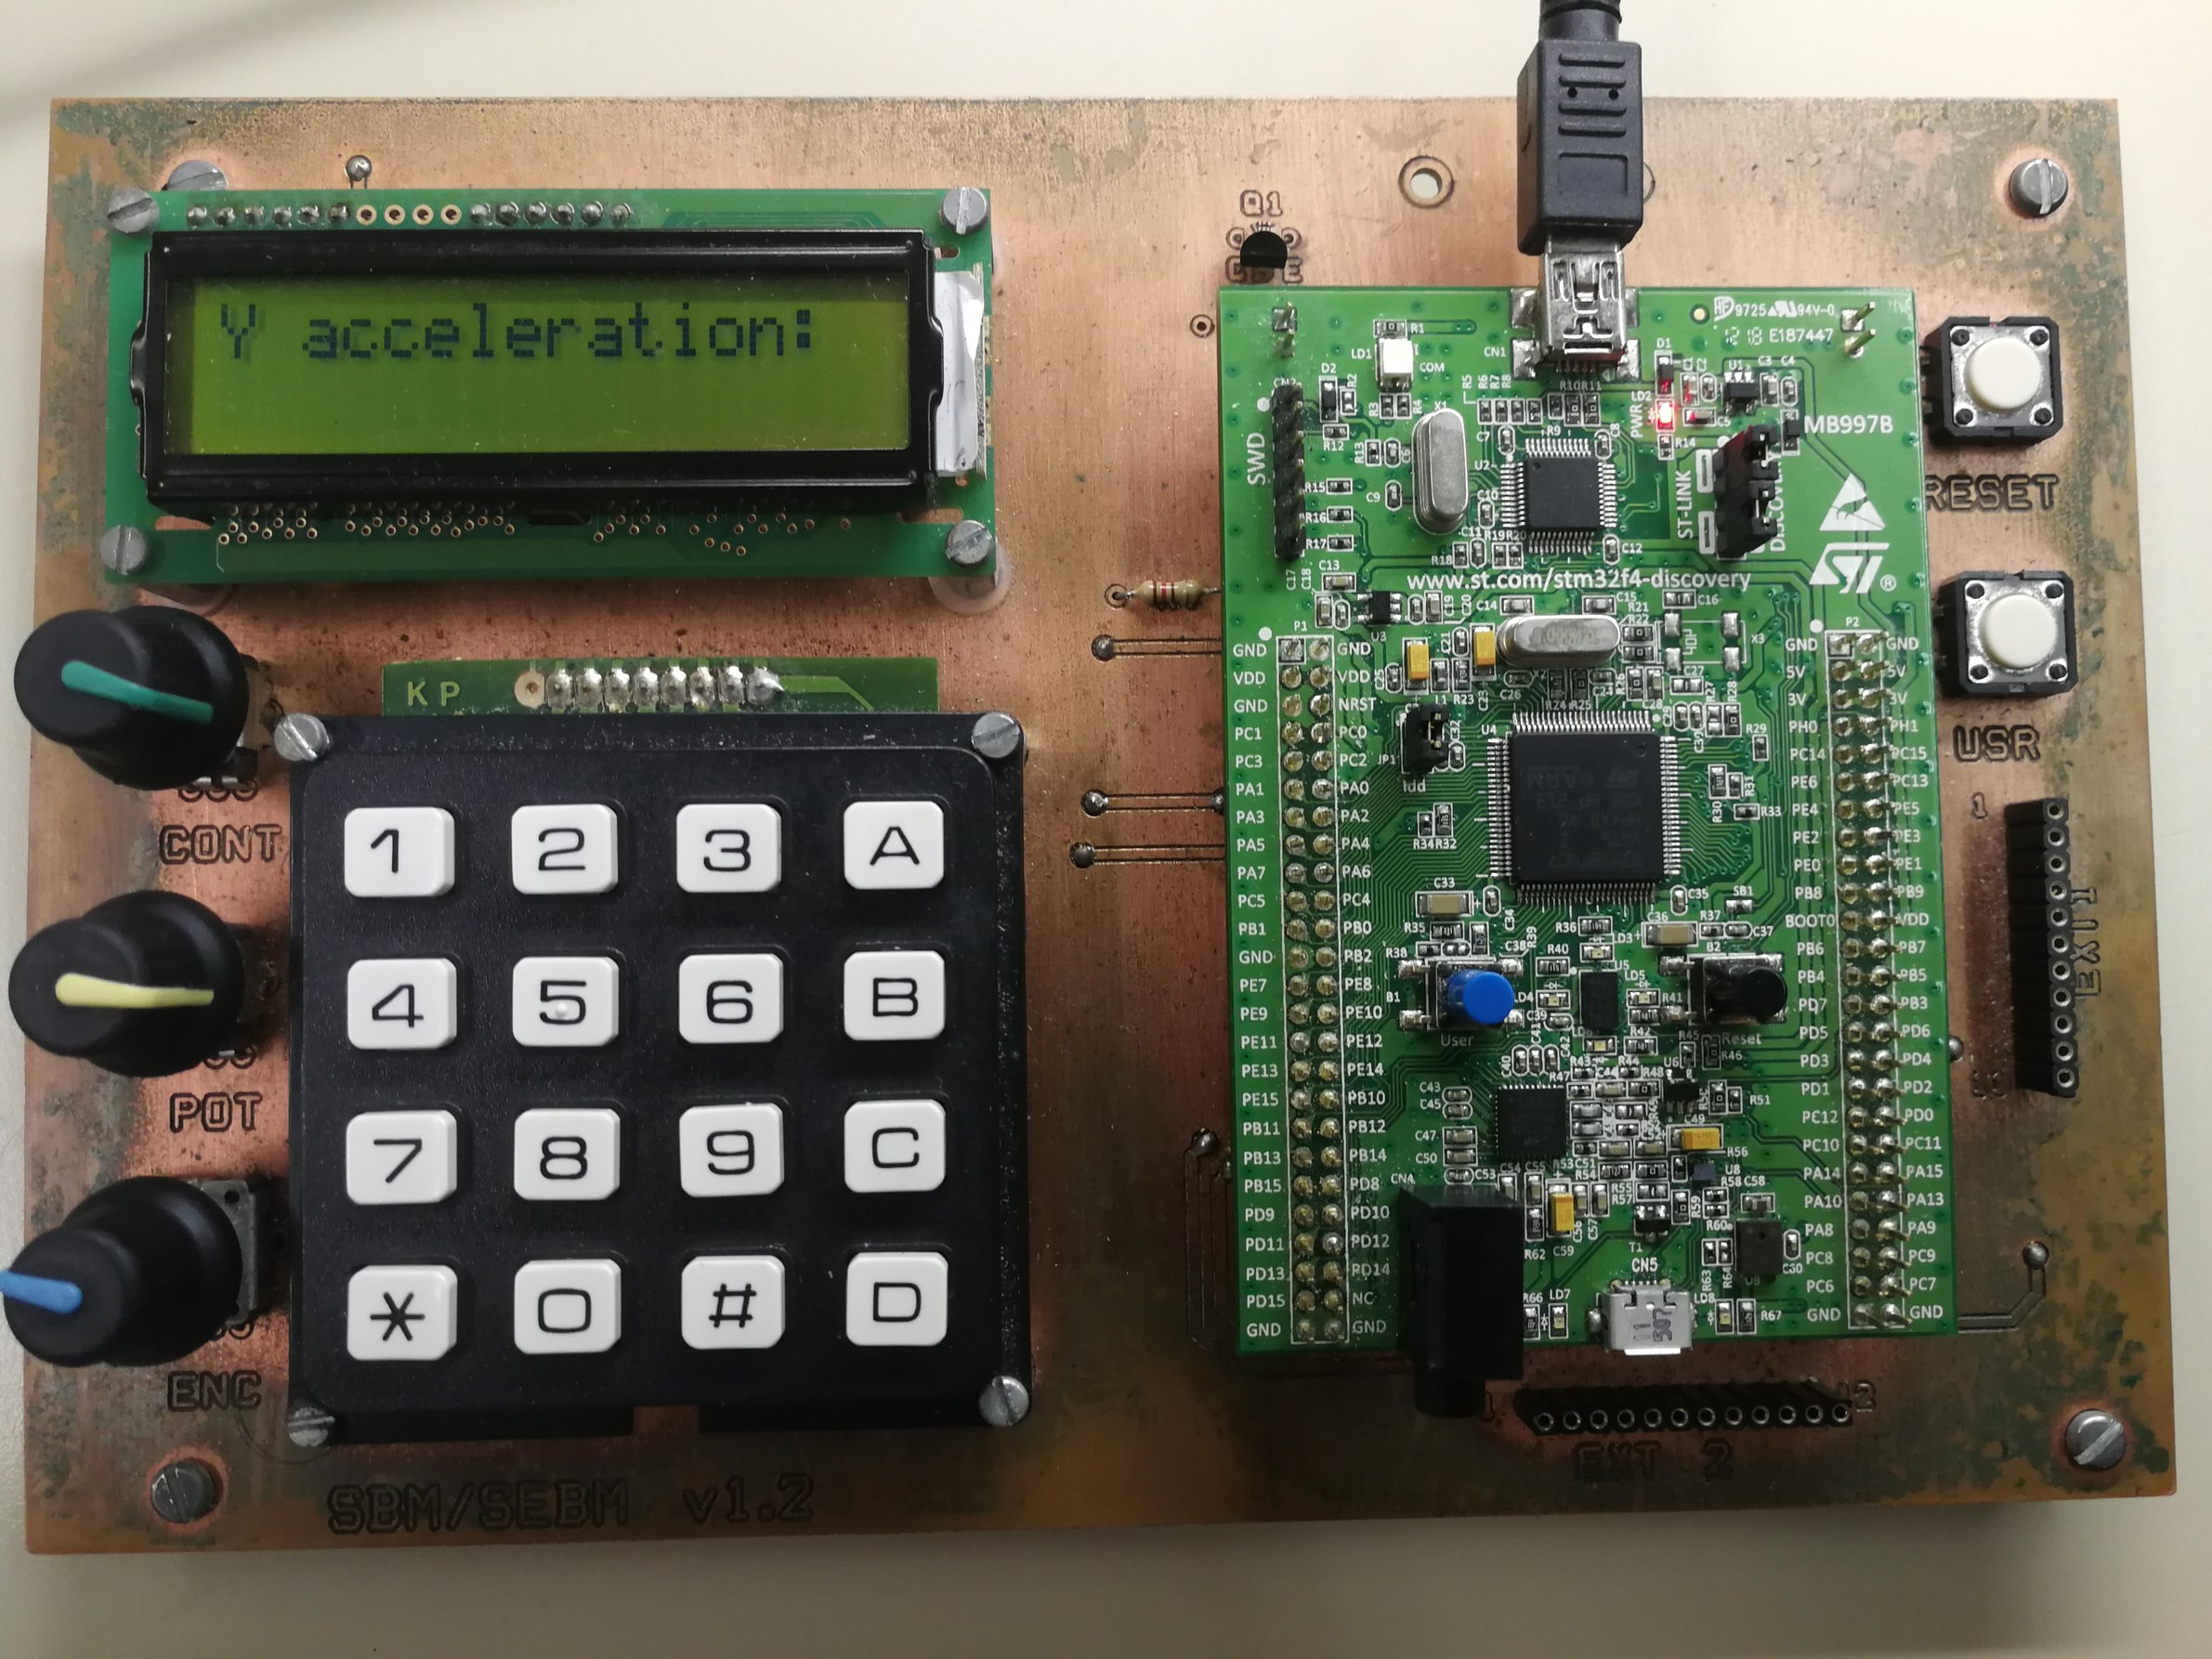
\includegraphics[width=.82\columnwidth]{../photos/board/p4-interrupt-initial}
  \caption{ \label{fig:p4-board-initial} La placa executant la prova d'interrupció, en l'estat inicial. }
\end{figure}
\begin{figure}[p]
  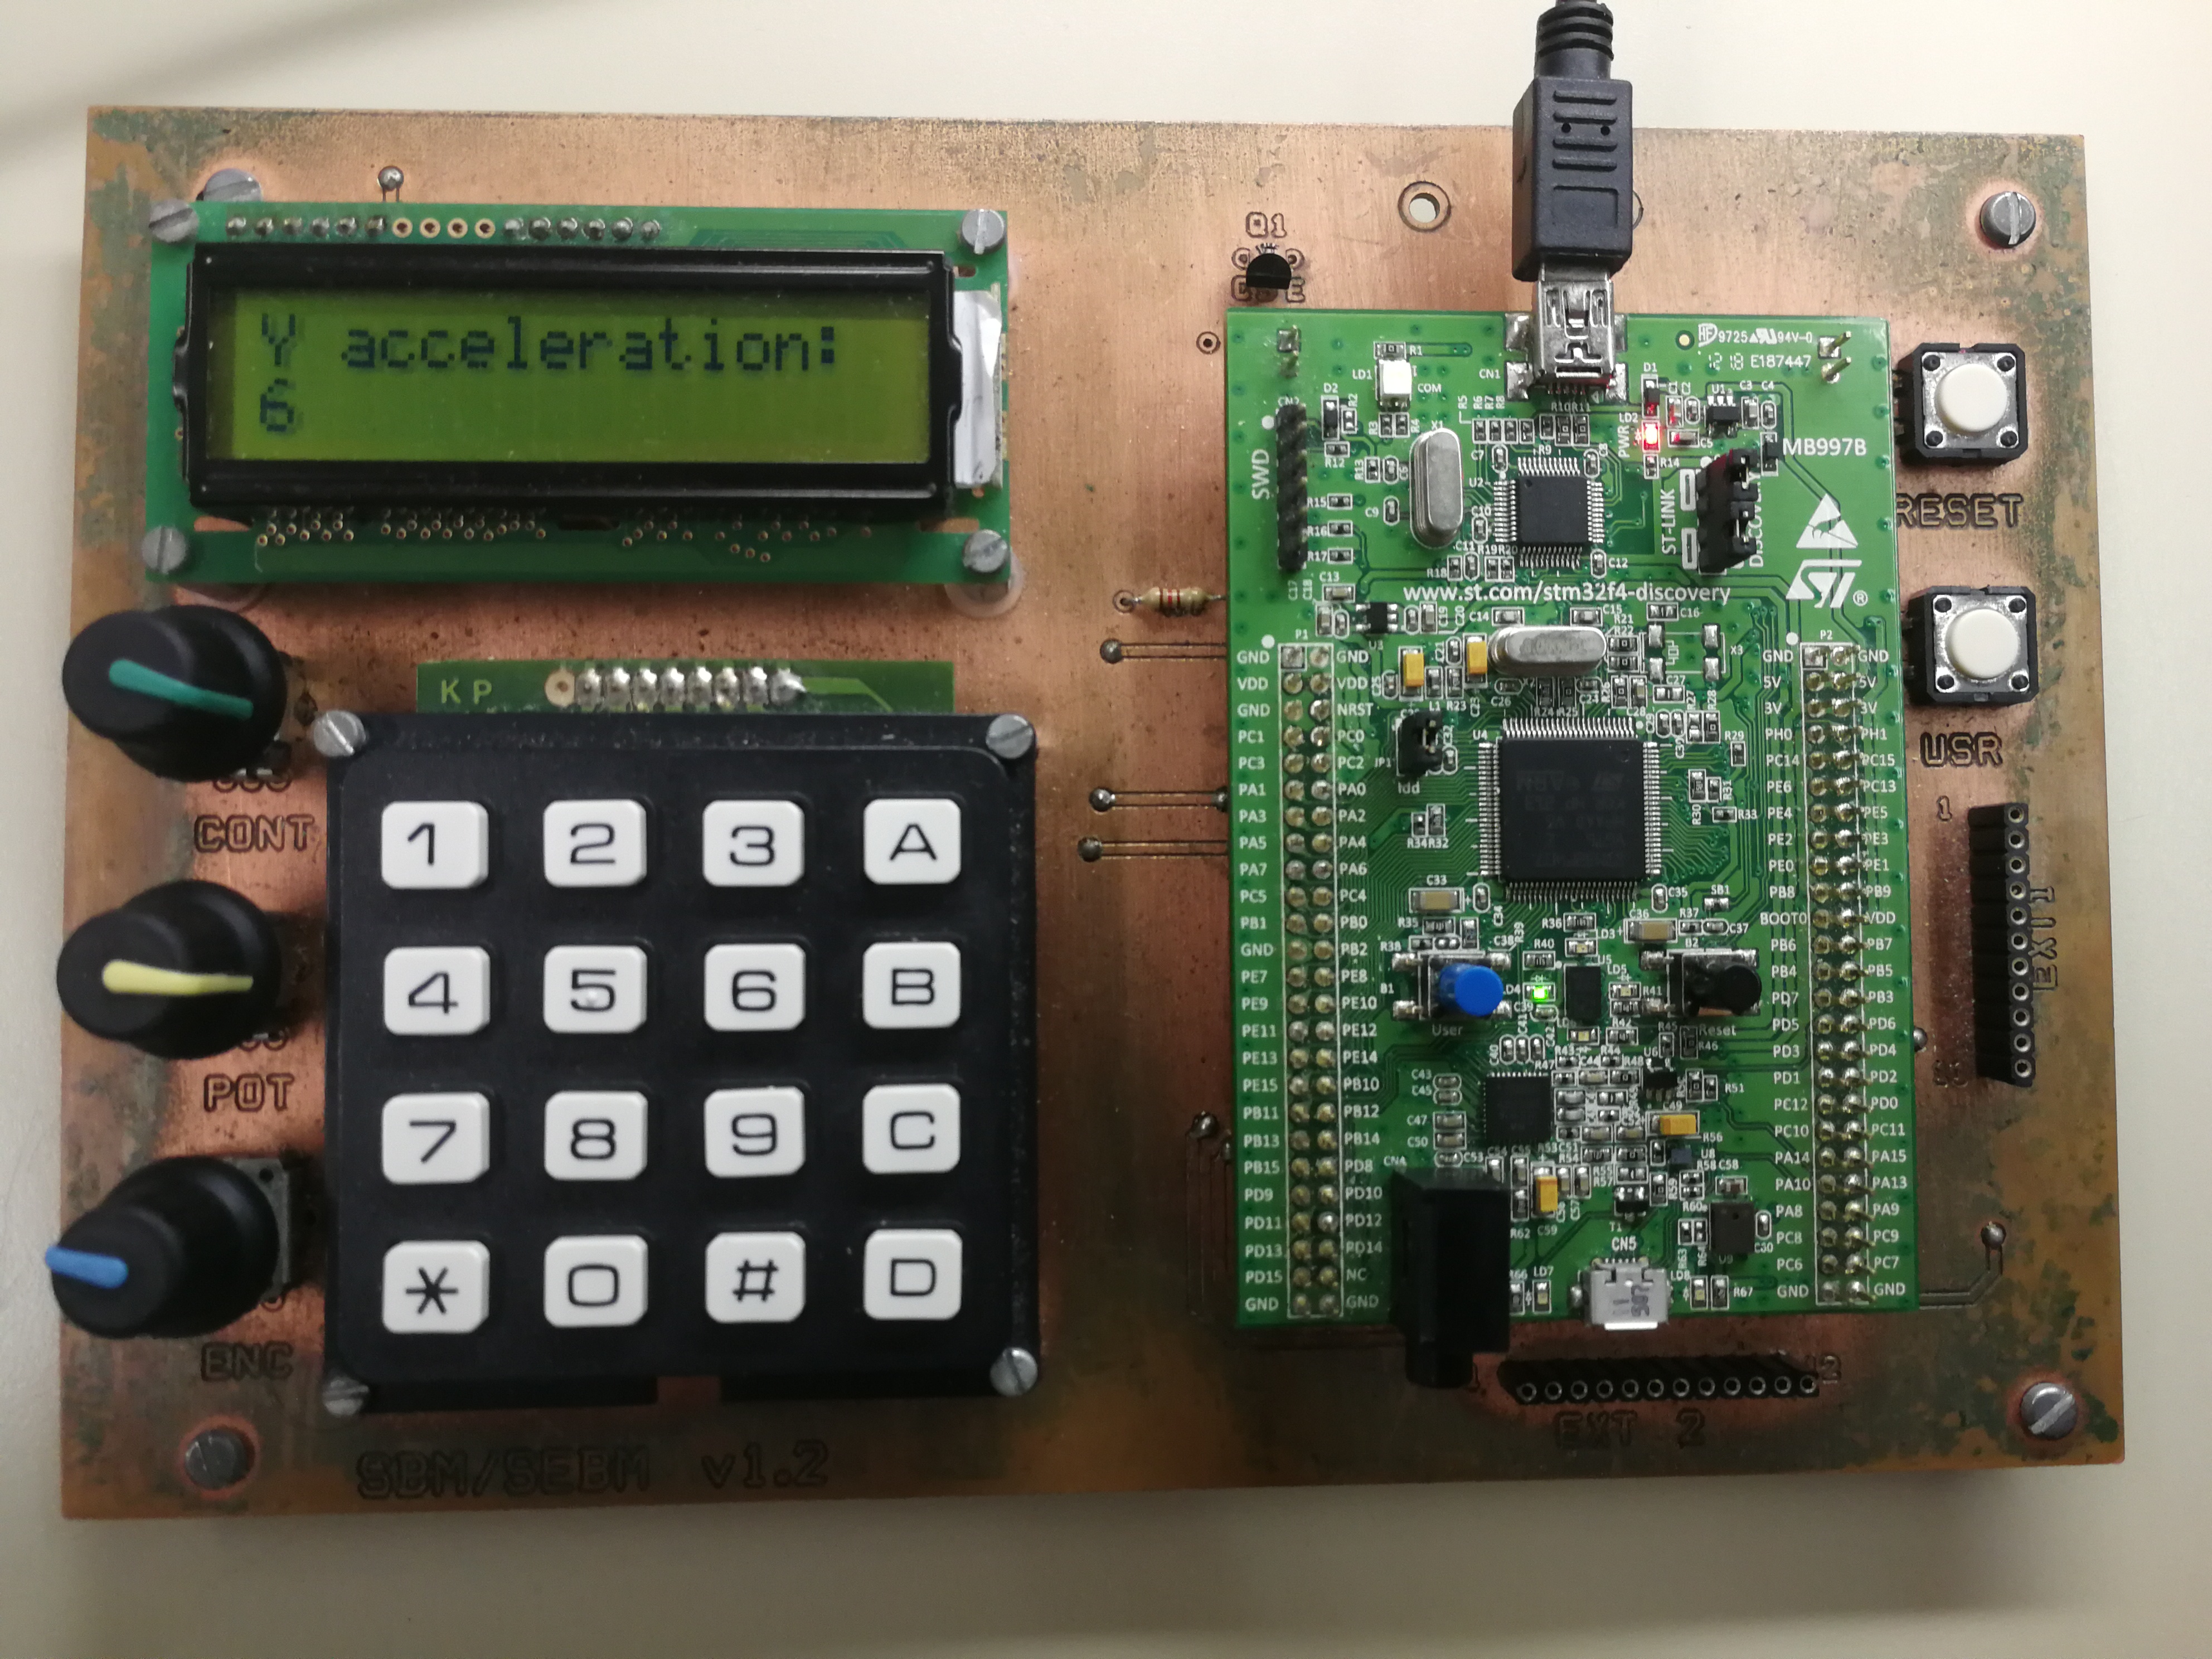
\includegraphics[width=.82\columnwidth]{../photos/board/p4-interrupt-use}
  \caption{ \label{fig:p4-board-use} La placa executant la prova d'interrupció, després de prémer el polsador. }
\end{figure}

El resultat es pot veure a les figures \ref{fig:p4-board-initial} (estat inicial) i
\ref{fig:p4-board-use} (després de premer el polsador d'usuari).
Es comprova el correcte funcionament del programa.


\subsection{Mesures de temporització}

Es comença ara amb l'analitzador lògic. En primer lloc mesurarem la latència d'interrupció
aproximada, mirant el temps que passa des de que demanem la interrupció (premem el polsador) fins que
aquesta s'executa (LED verd canvia d'estat).

Connectem i configurem l'analitzador com es demana.
En la figura~\ref{fig:p4-analyzer-latency} es pot veure que la latència d'interrupció és de
\SI{275}{\nano\second}.

\begin{figure}
  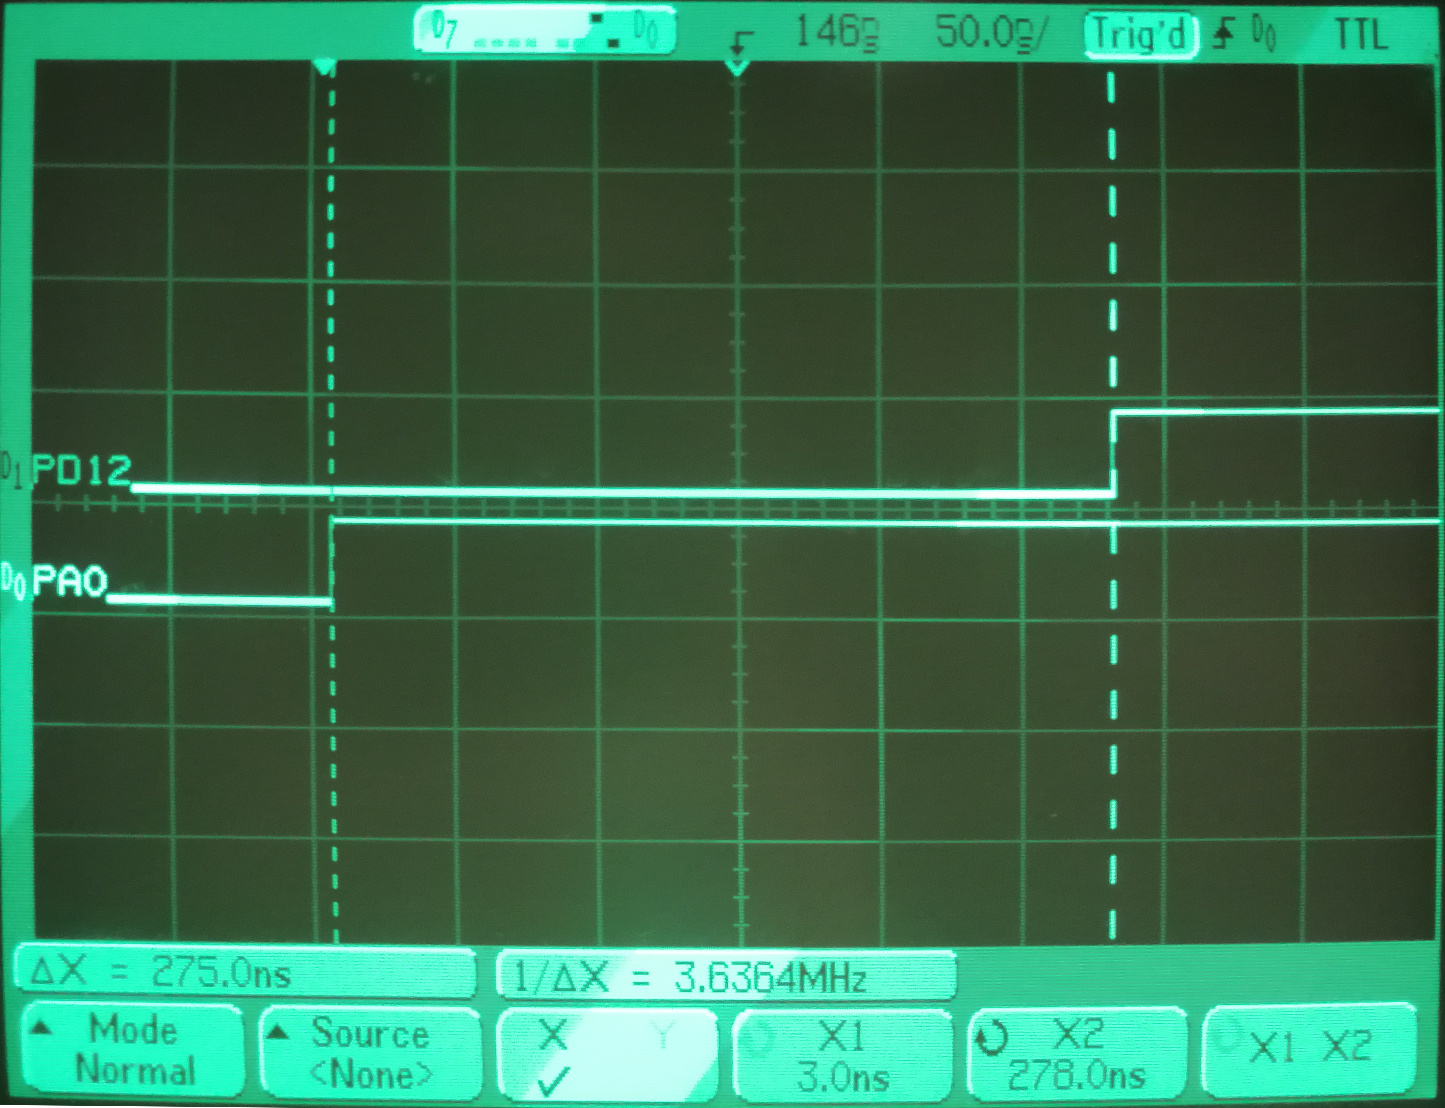
\includegraphics[width=.99\columnwidth]{../photos/analyzer/interrupt-latency}
  \caption{ \label{fig:p4-analyzer-latency} Captura mostrant la latència aproximada d'interrupció. }
\end{figure}

Es demana ara fer verificacions temporals del bus SPI. Com que en premer el polsador es fa
una lectura d'un registre, tenim una forma senzilla de capturar aquesta transferència SPI.
El cronograma d'una transferència per l'acceleròmetre LIS302DL es pot veure a la
figura~\ref{fig:p4-timing-accel}, i els requisits que s'han de complir es troben a la
figura~\ref{fig:p4-timing-accel-specs}. Es demana que verifiquem els valors de \textsf{fc(SPC)},
de \textsf{tsu(CS)}, de \textsf{tsu(SI)} i \textsf{th(SI)}, de \textsf{tv(SO)} i \textsf{th(SO)}
i també mirar que el valor de la línia \textsf{MOSI} representa una petició de lectura
del registre d'acceleració Y.

\begin{figure}
  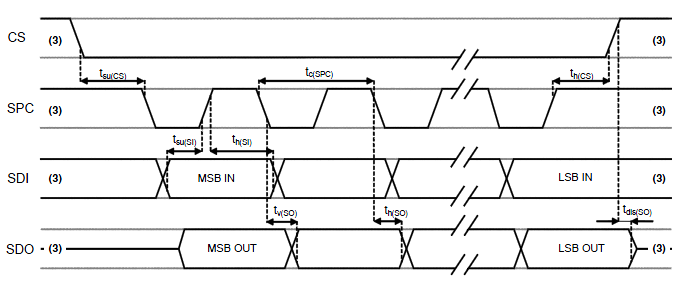
\includegraphics[width=0.8\columnwidth]{../\projectname/timing-accel-spi}
  \caption{ \label{fig:p4-timing-accel} Cronograma d'una transferència SPI a l'acceleròmetre. }
\end{figure}

\begin{figure}
  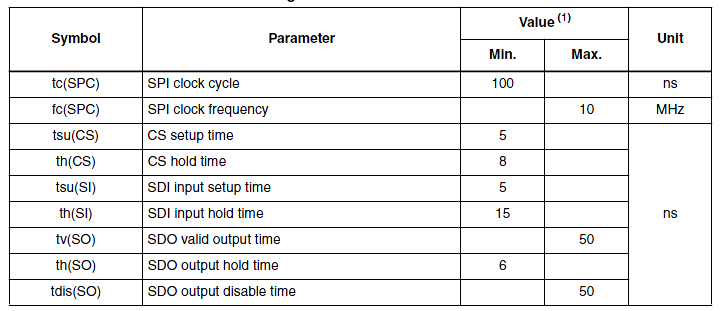
\includegraphics[width=0.85\columnwidth]{../\projectname/timing-accel-spi-specs}
  \caption{ \label{fig:p4-timing-accel-specs} Requeriments temporals per a una trasferència SPI a l'acceleròmetre. }
\end{figure}

En primer lloc configurem l'analitzador com es demana i capturem una lectura sencera de
l'acceleròmetre des de que es prem el polsador.
El resultat es pot veure a la figura~\ref{fig:p4-analyzer-overview}.
Comprovem que es compleix el protocol esperat.

\begin{figure}
  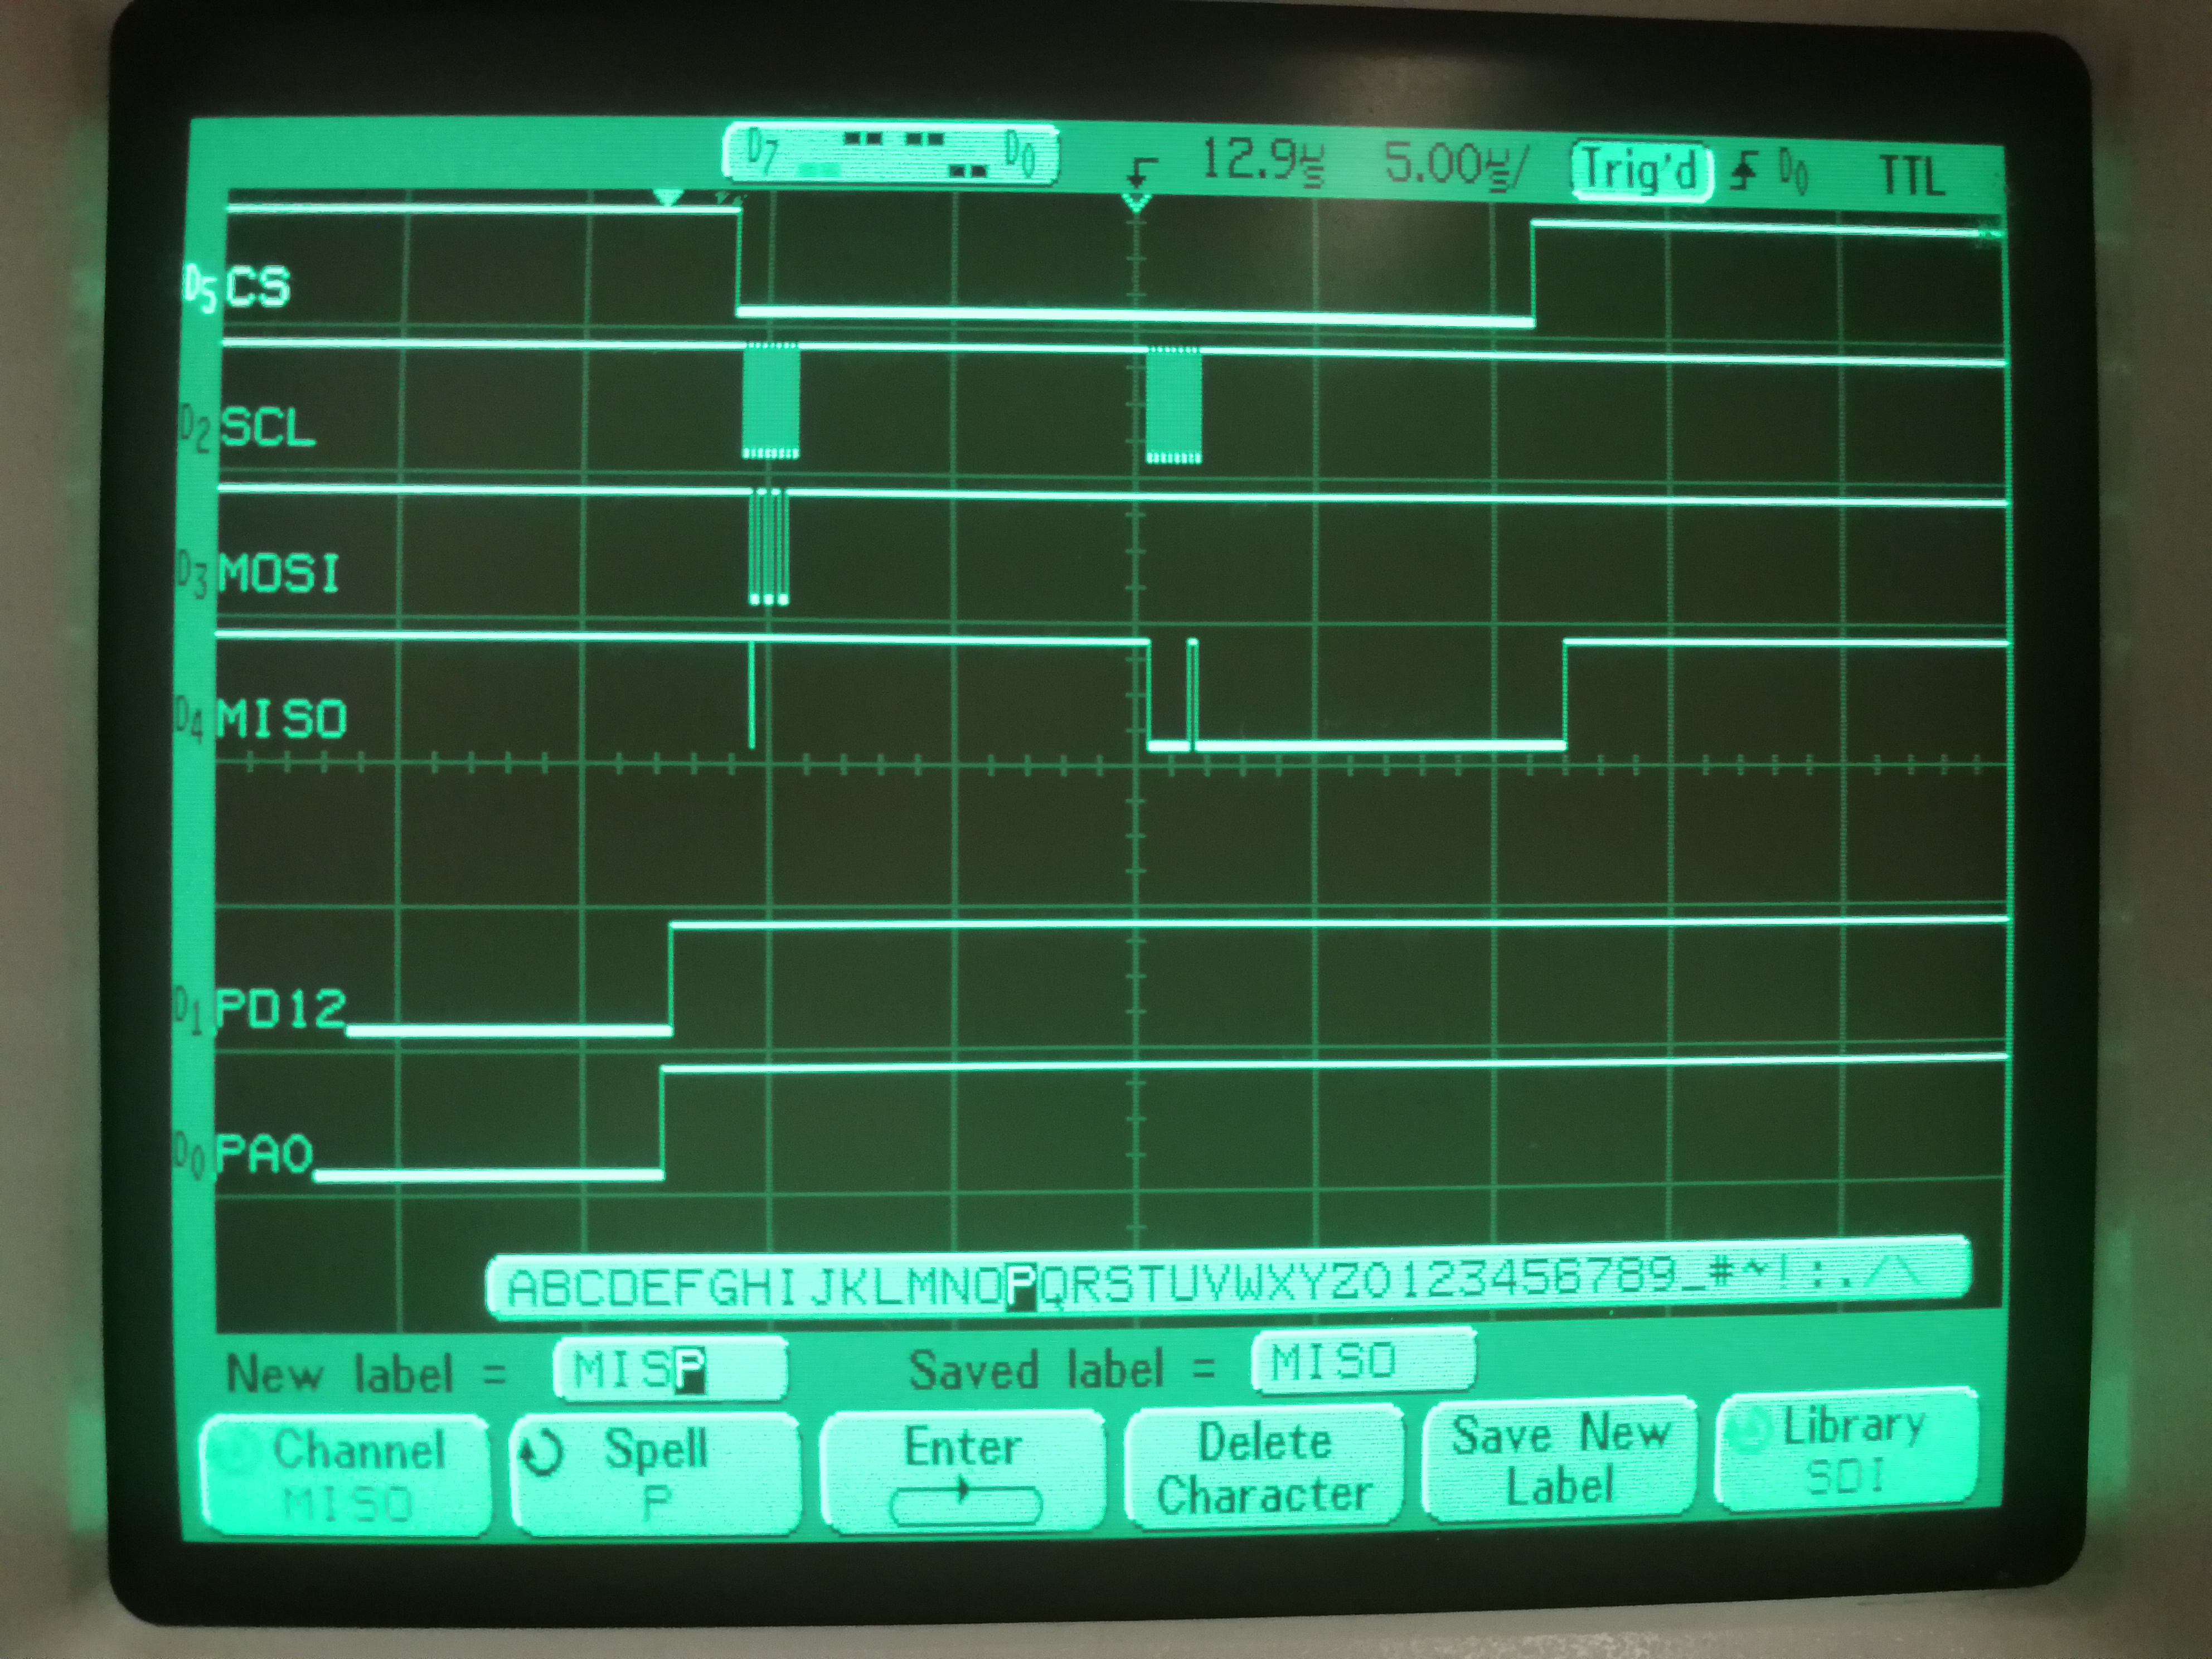
\includegraphics[width=.99\linewidth]{../photos/analyzer/interrupt-overview}
  \caption{ \label{fig:p4-analyzer-overview} Captura mostrant una lectura sencera de l'acceleròmetre des de que es prem el polsador d'usuari. }
\end{figure}

Ara realitzem les mesures concretes demanades a dalt.

A la figura~\ref{fig:p4-analyzer-transfers}
es poden veure de més a prop les dues transferències SPI que comporten la lectura.
A la figura~\ref{fig:p4-analyzer-cmd} es visualitza només una d'elles.

\begin{figure}
  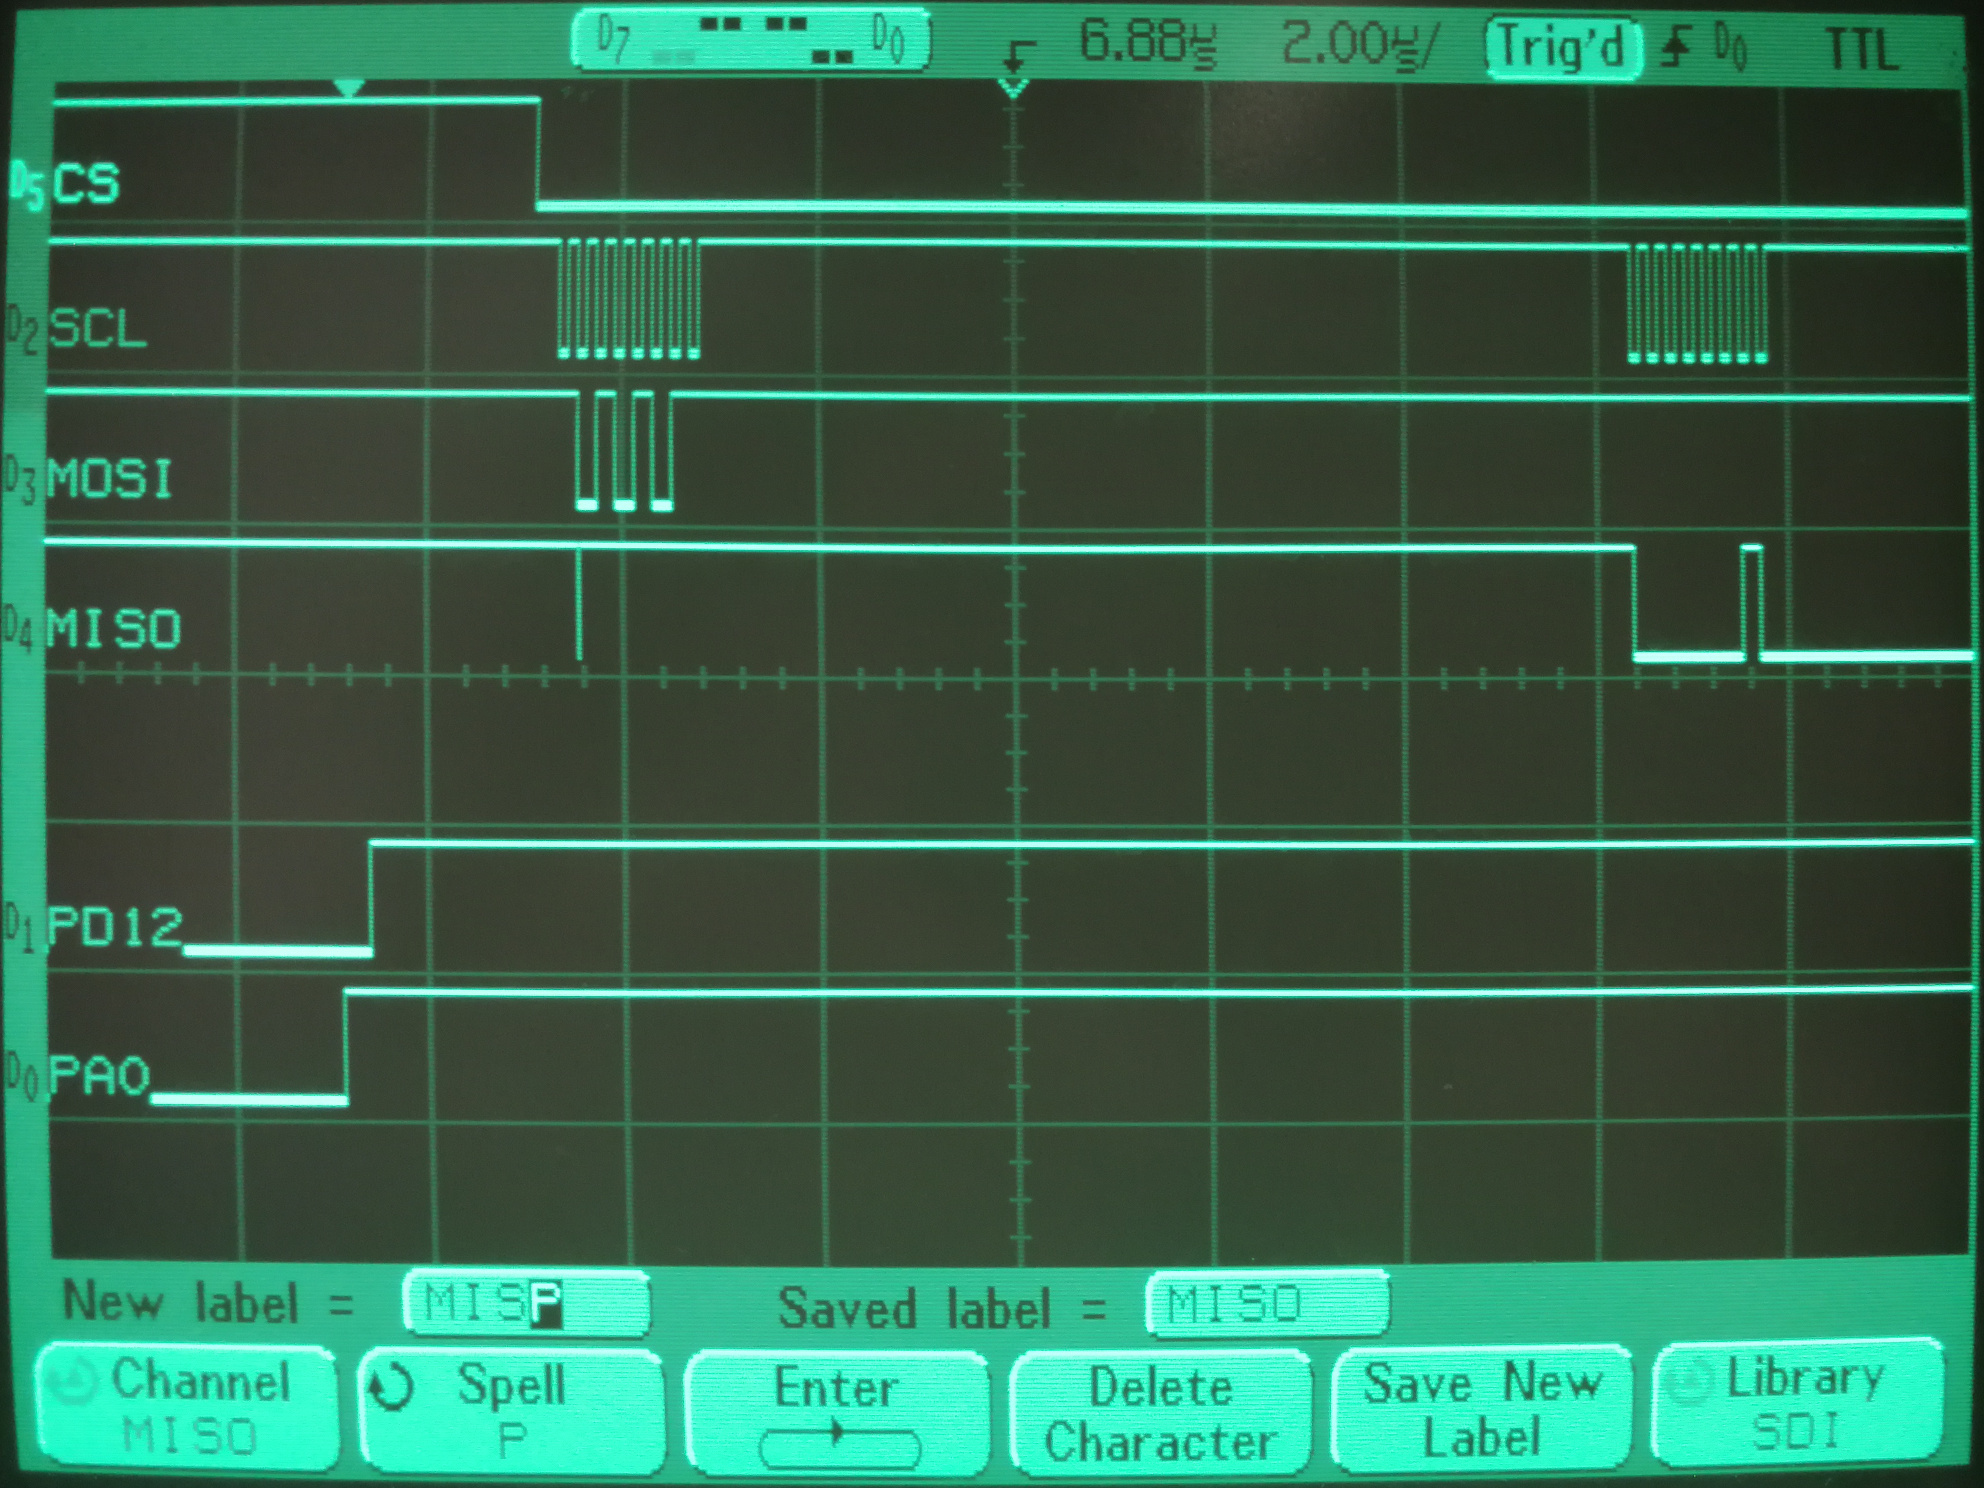
\includegraphics[width=.99\columnwidth]{../photos/analyzer/interrupt-accel}
  \caption{ \label{fig:p4-analyzer-transfers} Captura mostrant les dues transferències SPI que conformen una lectura a l'acceleròmetre. }
\end{figure}

\begin{figure}
  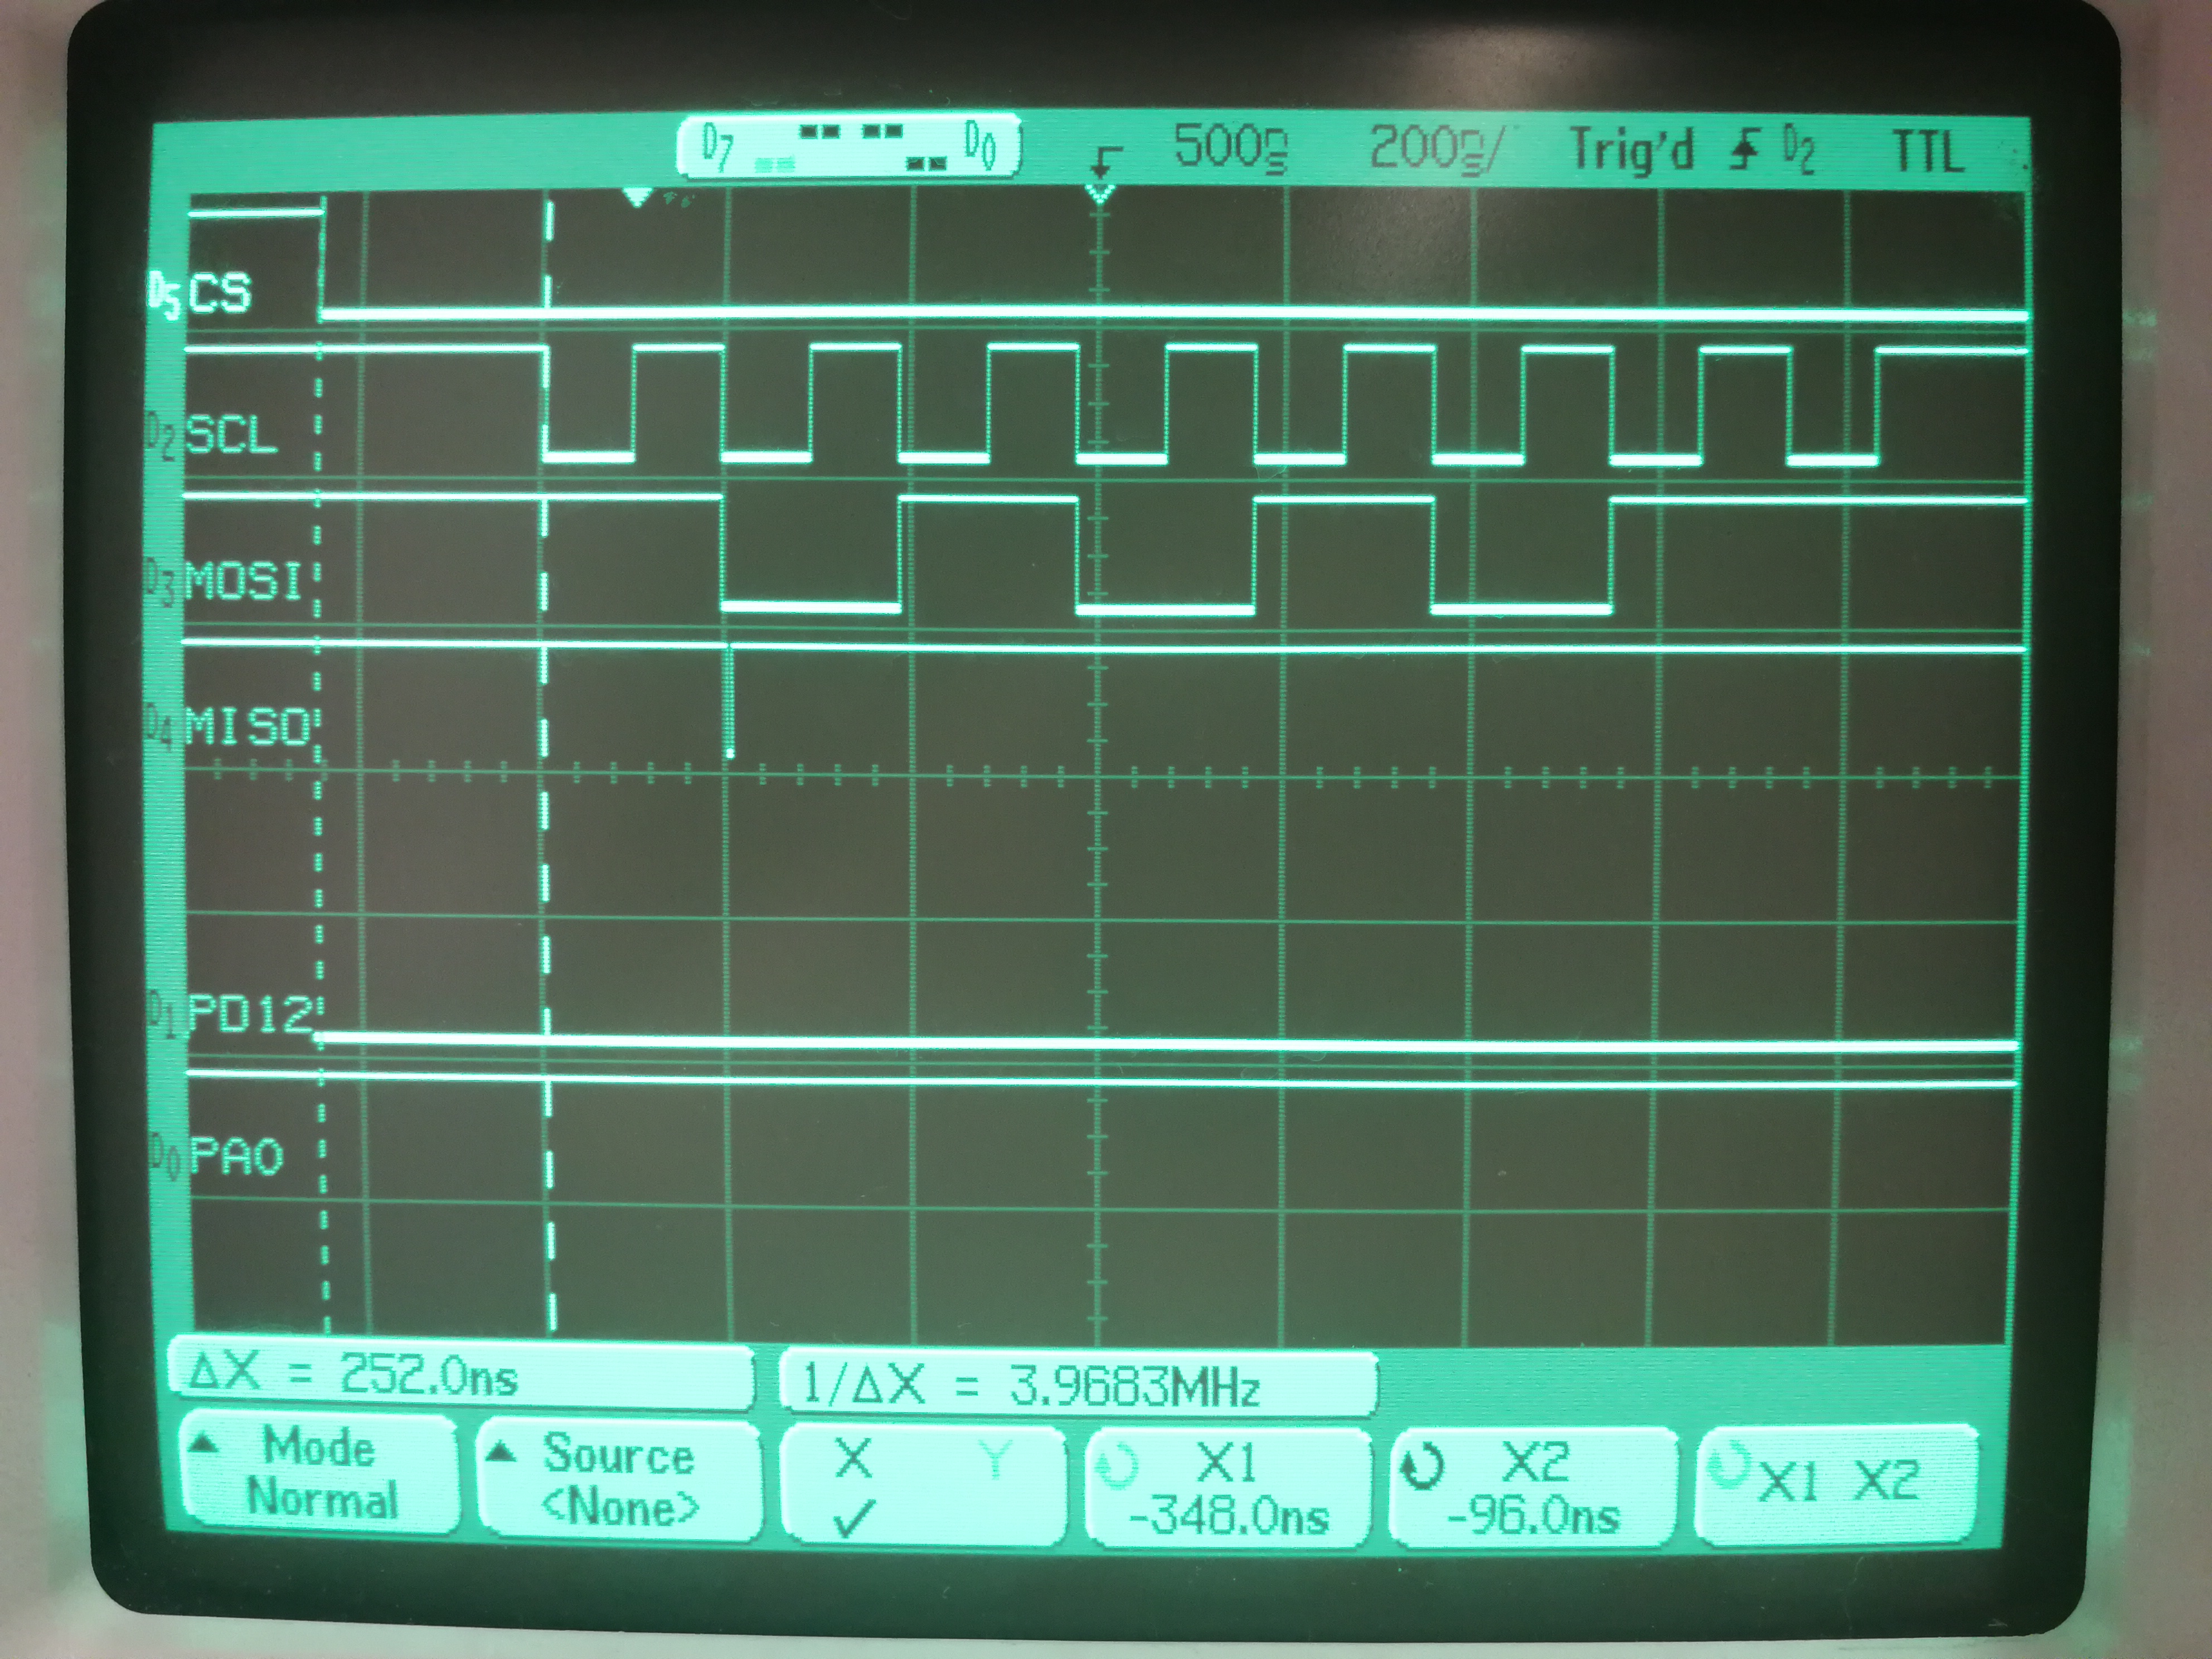
\includegraphics[width=.99\columnwidth]{../photos/analyzer/interrupt-accel-cmd}
  \caption{ \label{fig:p4-analyzer-cmd} Captura mostrant una transferència SPI cap a l'acceleròmetre on es fa una petició de lectura del registre de l'eix Y. }
\end{figure}

Les mesures de temporització són:

\begin{align*}
  \mathsf{fc(SPC)} &= \frac{1}{\SI{192}{\nano\second}} \simeq \SI{5.21}{\mega\hertz}
\\
  \mathsf{tsu(CS)} &= \SI{252}{\nano\second}
\\
  \mathsf{tsu(SI)} &= \SI{93}{\nano\second}
\\
  \mathsf{th(SI)} &= \SI{94}{\nano\second}
\\
  \mathsf{tv(SO)} &= \SI{9}{\nano\second}
\\
  \mathsf{th(SO)} &= \SI{6}{\nano\second}
\end{align*}

Tot està dins les especificacions esperades. També comprovem que el valor que es transmet cap a l'esclau
és un \mintinline{c}|0b10101011|, per tant $\mathsf{R}/\overline{\mathsf{W}} = 1$ (lectura), $\mathsf{M}/\overline{\mathsf{S}} = 0$ (manual), registre 101011 (\mintinline{c}|0x2B|, OutY). Per tant, tot correcte també.


\clearpage
\subsection{\label{sub:p4-lcd} Temporització de l'LCD}

\opcional
La realització d'aquesta secció és opcional.

Ara es demana fer verificacions temporals sobre el codi de l'LCD. En primer lloc, volem
comprovar que quan realitzem una escriptura a l'LCD (veure cronograma en la 
figura~\ref{fig:p2-timing-write}, pàgina~\pageref{fig:p2-timing-write}) es compleixen les
especificacions del \emph{datasheet} (figura~\ref{fig:p4-timing-lcd-specs})).

\begin{figure}
  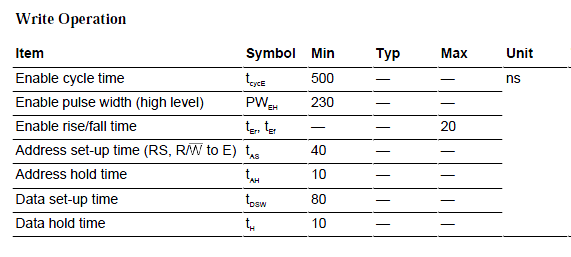
\includegraphics[width=0.85\columnwidth]{../\projectname/timing-lcd-specs}
  \caption{ \label{fig:p4-timing-lcd-specs} Requeriments temporals per a una escritura a l'LCD. }
\end{figure}

En concret, volem comprovar que es compleixen els valors de $t_{AS}$, $t_{AH}$, $t_{DSW}$, $t_H$ i $P_{WEH}$.

Configurem l'analitzador lògic adequadament, i fem la captura d'una transferència, que es pot
veure en la figura~\ref{fig:p4-analyzer-lcd-write}.

\begin{figure}
  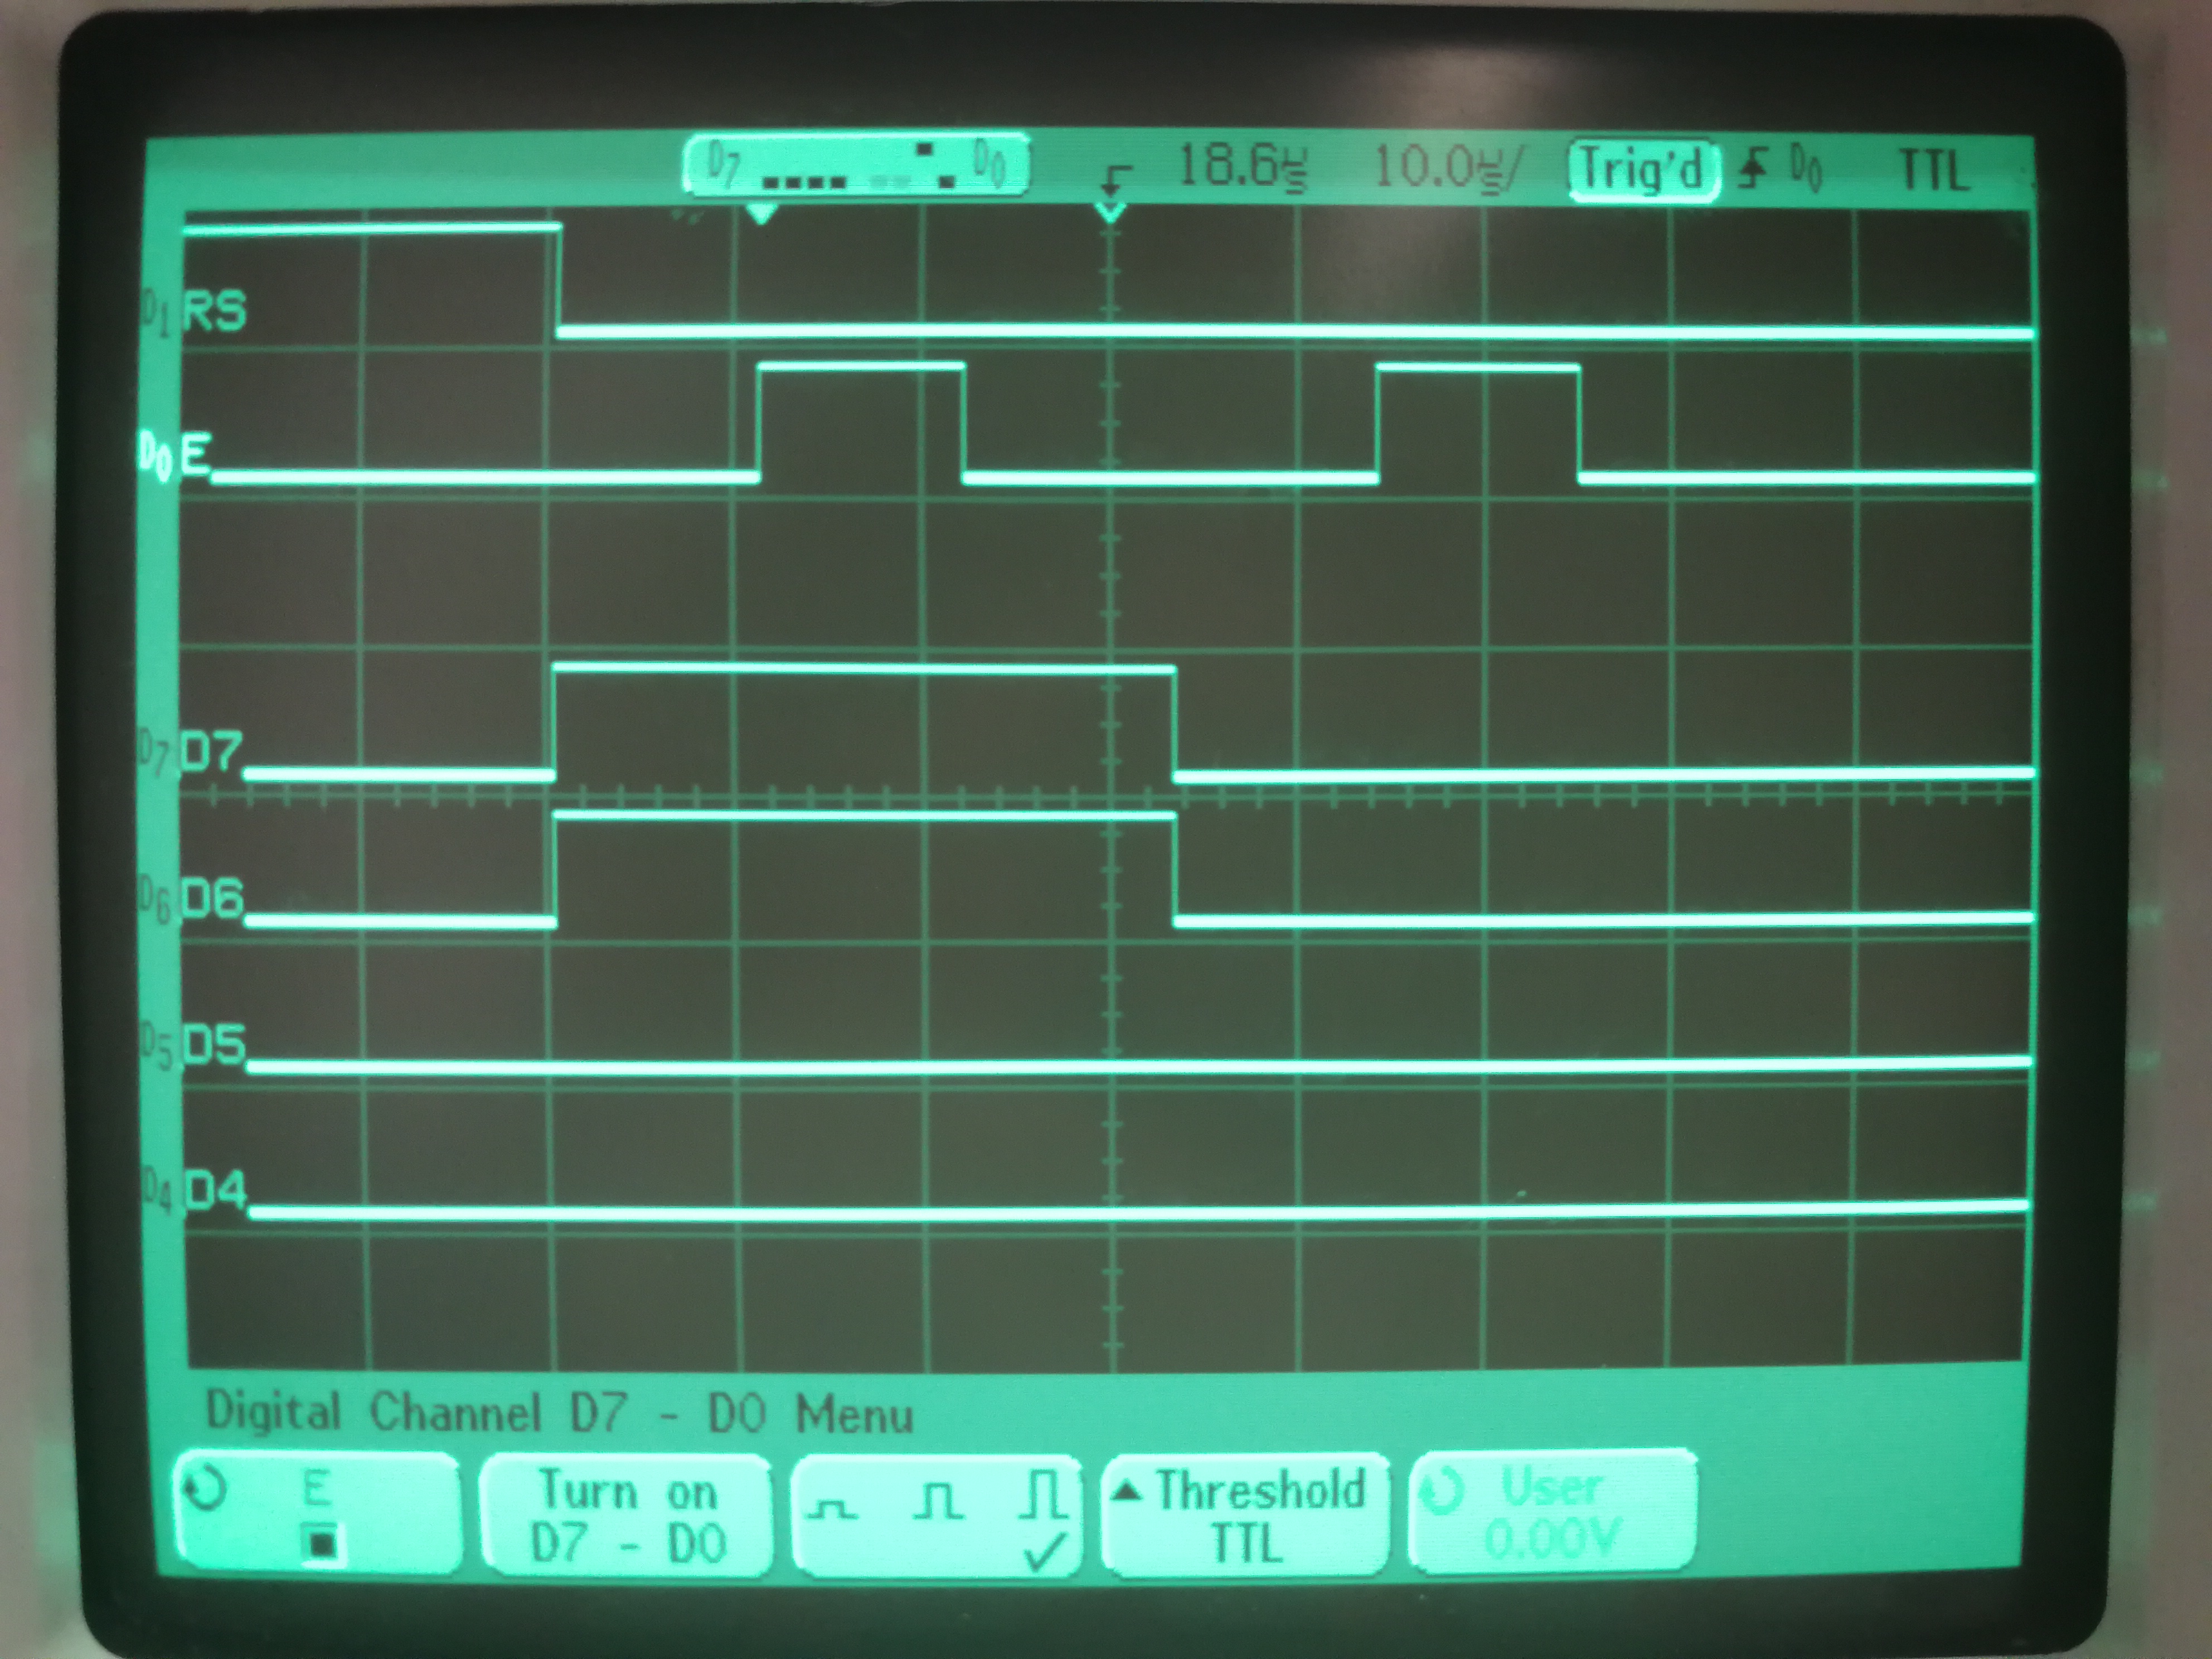
\includegraphics[width=.99\columnwidth]{../photos/analyzer/lcd-write}
  \caption{ \label{fig:p4-analyzer-lcd-write} Captura mostrant una única transferència d'escriptura cap a l'LCD. }
\end{figure}

Les mesures realitzades son:

\begin{align*}
  t_{AS} &= \SI{10.8}{\micro\second}
\\
  t_{AH} &= \SI{11.1}{\micro\second}
\\
  t_{DSW} &= \SI{21.8}{\micro\second}
\\
  t_{H} &= \SI{11.1}{\micro\second}
\\
  P_{WEH} &= \SI{10.8}{\micro\second}
\end{align*}

Comprovem que respecta les especificacions.

Ara capturarem la seqüència d'inicialització de
l'LCD i comprovarem que es respecta el protocol exposat en la pàgina~\pageref{sub:p2-init},
que es pot veure en la figura~\ref{fig:p2-init-protocol}.

Començarem extraient una captura del procés d'inicialització en general, que es pot veure
en la figura~\ref{fig:p4-analyzer-lcd-init}. Podem veure primer un glitch, i \SI{10}{\milli\second}
després, com s'inicialitzen els pins GPIO i es posen tots a zero. \SI{50}{\milli\second} després
s'envia la primera comanda a l'LCD (0011), llavors s'espera \SI{10}{\milli\second} i es repeteix seguida
d'una petita espera i la resta de comandes d'inicialització. Un cop fet el protocol,
el codi espera \SI{5}{\milli\second} i fa 4 comandes (8 escriptures) per escriure OK a l'LCD.

\begin{figure}
  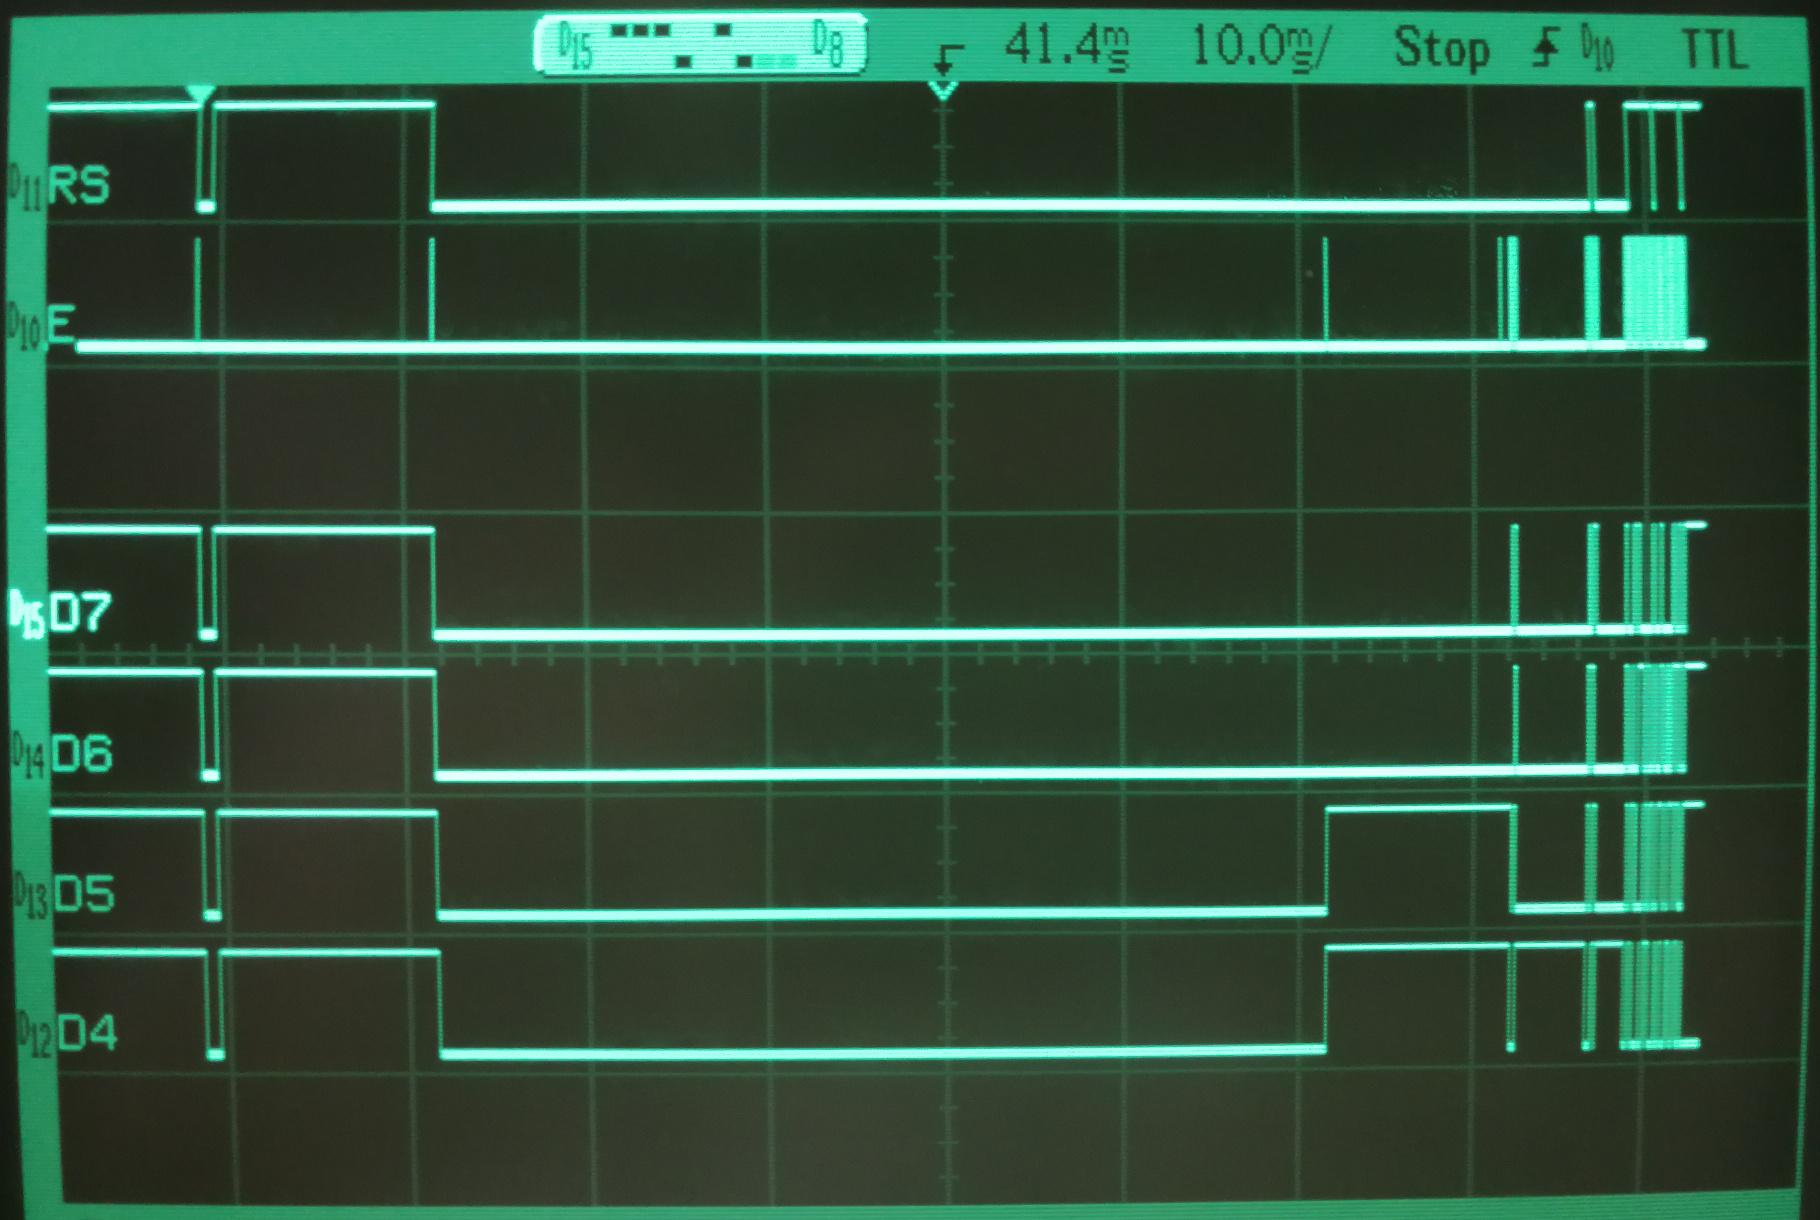
\includegraphics[width=.99\columnwidth]{../photos/analyzer/lcd-init-full-1}
  \caption{ \label{fig:p4-analyzer-lcd-init} Captura mostrant el procés d'inicialització de l'LCD sencer. }
\end{figure}

Per tant, veiem que el codi d'inicialització respecta les esperes. Ara farem una captura només de la part
on es fan escritures, és a dir, des de quan s'envia el primer 0011 (després d'esperar \SI{50}{\milli\second}) fins
que s'acaba d'escriure OK. La captura es pot veure a la figura~\ref{fig:p4-analyzer-lcd-protocol}.

\begin{figure}
  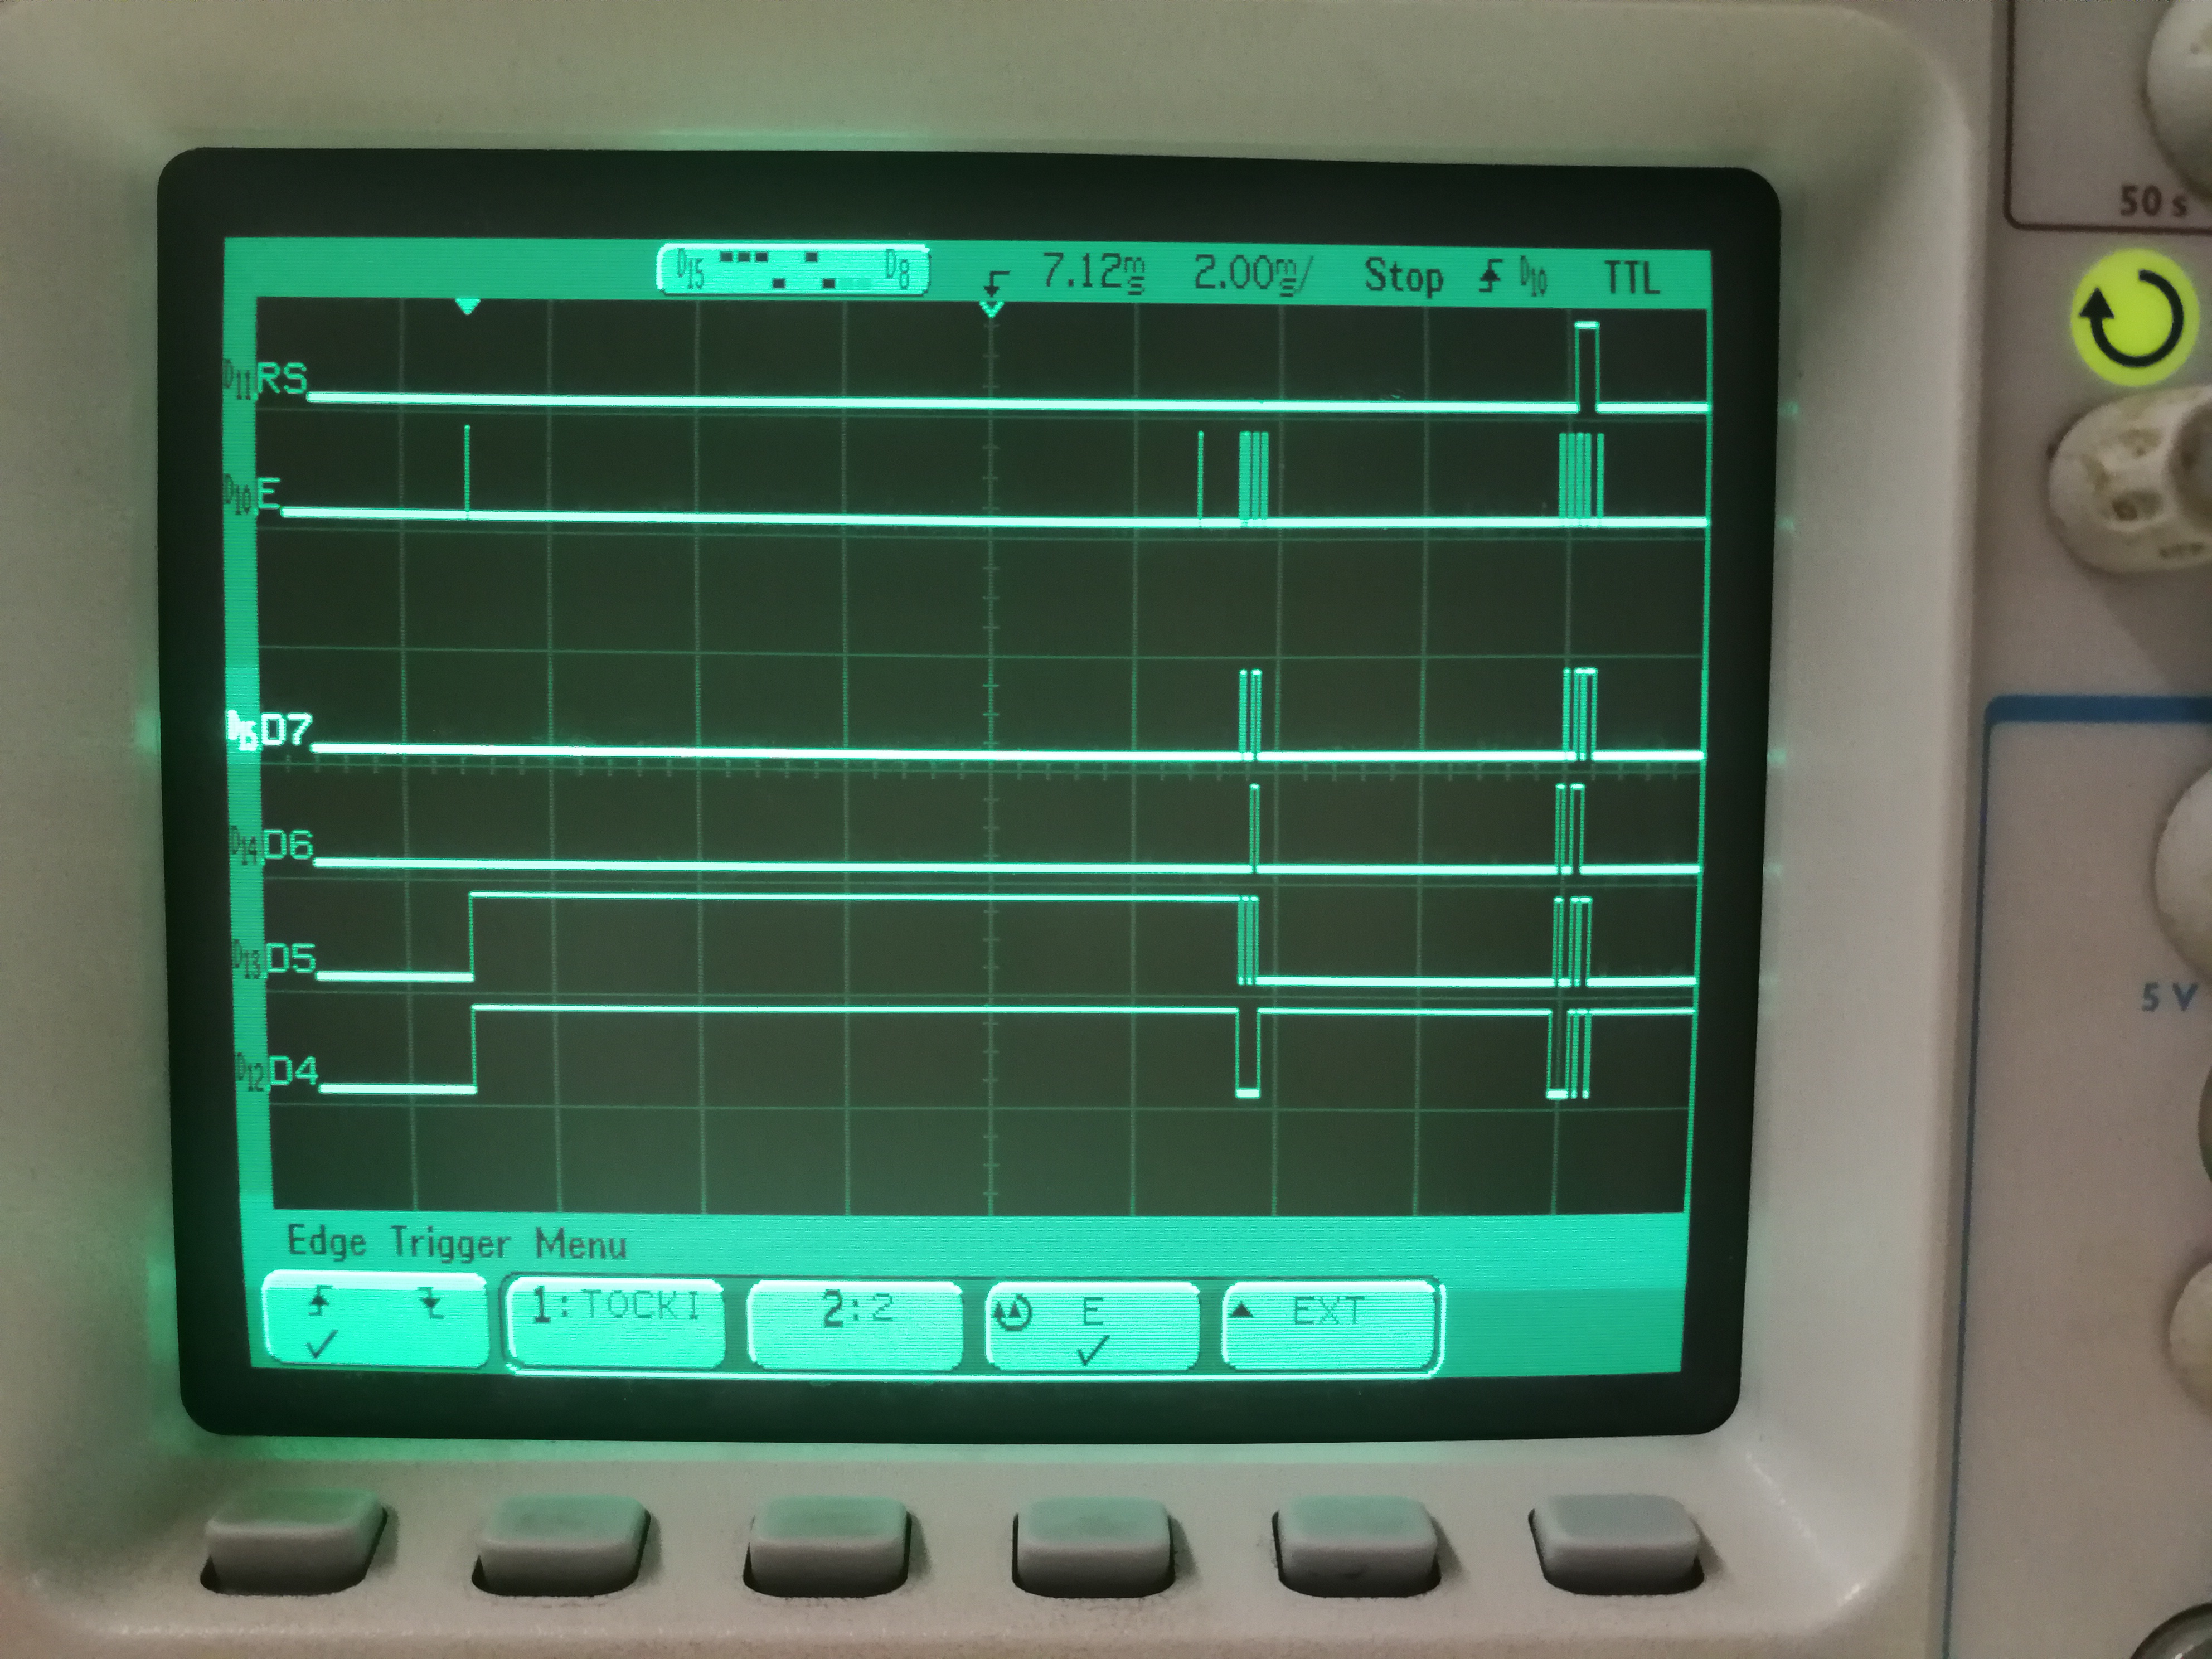
\includegraphics[width=.99\columnwidth]{../photos/analyzer/lcd-init-z1}
  \caption{ \label{fig:p4-analyzer-lcd-protocol} Captura mostrant les escritures d'inicialització de l'LCD. }
\end{figure}

Comencem a verificar que les comandes son les correctes i ens trobem un error.
Aquest es pot veure a la figura~\ref{fig:p4-analyzer-lcd-protocol-zoom}, on s'ha ampliat
la captura per veure concretament les escriptures que demana la \emph{datasheet} que fem
(figura de la pàg.~\pageref{fig:p2-init-protocol}).

\begin{figure}
  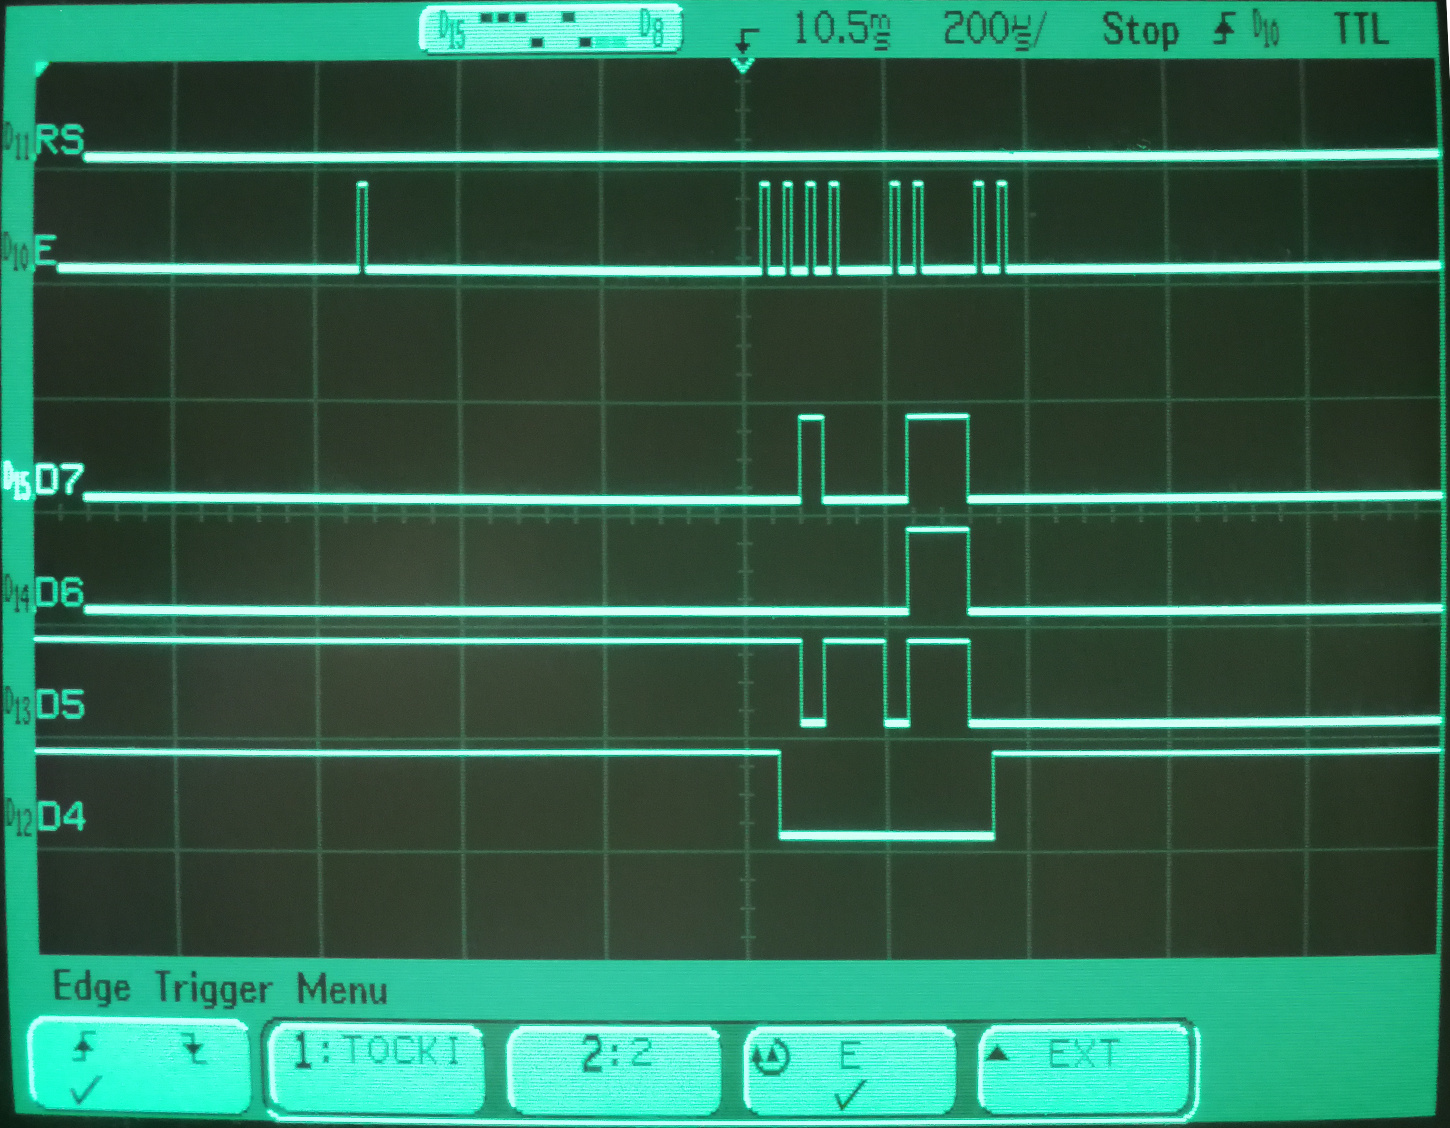
\includegraphics[width=.99\columnwidth]{../photos/analyzer/lcd-init-z2}
  \caption{ \label{fig:p4-analyzer-lcd-protocol-zoom} Captura mostrant les últimes escritures del protocol d'inicialització de l'LCD. }
\end{figure}

En la figura podem veure la segona escriptura 0011, l'espera de \SI{500}{\micro\second} i l'últim bloc
d'escriptures que es demana. Les escriptures d'aquest últim bloc son:

\begin{minted}{text}
0011
0010
1000 0010
0000 1110
0000 0001
\end{minted}
\vskip -1em

Mentre que les escriptures demanades al datasheet (en el nostre cas $I/D = 1; S = 0$ i tenim un display de dues línies, per tant $N = 1$ i $F$ no importa):

\begin{minted}{text}
0011
0010
0010 1***
0000 1000
0000 0001
\end{minted}
\vskip -1em

D'entrada veiem que \textbf{la tercera i la quarta escriptura estan canviades de lloc}. Aquestes dues
escriptures (0010 1***) configuren les línies i el tipus de caràcters que té el display. En comptes d'això,
el codi està escrivint 1000 0010, que és una comanda \emph{Set DDRAM address} i situa el cursor en la posició
2 de la DDRAM.

Anem al codi i corregim el bug (\commit{d6babe86f524c875e7b5d9e93cf336c434c1b18c}):

\begin{minted}{diff}
--- a/lcd.c
+++ b/lcd.c
@@ -181,8 +181,8 @@ void LCD_Init(void) {
     lcdNibble(0x02, 0);
 
     // Mode 4 bits 2 lines 5x8 chars
-    lcdNibble(0x08, 0);
     lcdNibble(0x02, 0);
+    lcdNibble(0x08, 0);
     DELAY_US(50);
 
     // Display on blink on and cursor on
\end{minted}
\vskip -1em

També hi ha una segona diferència: la sisena escriptura és un 1110 en comptes d'un 1000. És a dir, en comptes
de la comanda original (apagar el display) que demana el datasheet, el codi l'encen i també activa el cursor.
Encara que no s'estigui seguint la inicialització com a tal, no hauria de causar cap comportament inesperat.

\textbf{Nota:} El \emph{datasheet} demana dues escritures més 0000 i 0110 al final, però no s'han inclós perquè es fan
després de l'espera i aquest comportament es considera correcte.


\section{Conclusió}

El major obstacle en aquesta pràctica ha estat aprendre a navegar per l'interfície d'usuari
de l'analitzador i les seves limitacions... També la dificultat de fer algunes mesures
que requerien posar-lo en mode \emph{one shot}. La part que més em preocupava (implementar
les interrupcions) no ha sigut problema.
%FIXME: conclusion

Ha estat molt satisfactori finalment corregir el bug de l'LCD!
Portava des del principi del curs investigant per què de vegades l'LCD només s'encenia amb una línia.

\section{Ajustaments posteriors}

Cap canvi a destacar.
% TODO
